\documentclass[review]{elsarticle}
%DIF LATEXDIFF DIFFERENCE FILE
%DIF DEL old.tex    Fri Jun  2 14:05:39 2023
%DIF ADD main.tex   Fri Jun  2 14:22:33 2023
\usepackage{hyperref}
\usepackage[margin=1in]{geometry}
\usepackage{graphicx}
\usepackage{amsmath}
\usepackage{placeins}
\usepackage{comment}
\usepackage{gensymb}
\usepackage{lineno}
\usepackage{color}
\usepackage{cleveref}
\usepackage{caption}
\usepackage{subcaption}

%\journal{Journal of Nuclear Materials}
\bibliographystyle{elsarticle-num}
%DIF PREAMBLE EXTENSION ADDED BY LATEXDIFF
%DIF CTRADITIONAL PREAMBLE %DIF PREAMBLE
\RequirePackage{color}\definecolor{RED}{rgb}{1,0,0}\definecolor{BLUE}{rgb}{0,0,1} %DIF PREAMBLE
\RequirePackage[stable]{footmisc} %DIF PREAMBLE
\DeclareOldFontCommand{\sf}{\normalfont\sffamily}{\mathsf} %DIF PREAMBLE
\providecommand{\DIFaddtex}[1]{{\protect\color{blue} \sf #1}} %DIF PREAMBLE
\providecommand{\DIFdeltex}[1]{{\protect\color{red} [..\footnote{removed: #1} ]}} %DIF PREAMBLE
%DIF SAFE PREAMBLE %DIF PREAMBLE
\providecommand{\DIFaddbegin}{} %DIF PREAMBLE
\providecommand{\DIFaddend}{} %DIF PREAMBLE
\providecommand{\DIFdelbegin}{} %DIF PREAMBLE
\providecommand{\DIFdelend}{} %DIF PREAMBLE
\providecommand{\DIFmodbegin}{} %DIF PREAMBLE
\providecommand{\DIFmodend}{} %DIF PREAMBLE
%DIF FLOATSAFE PREAMBLE %DIF PREAMBLE
\providecommand{\DIFaddFL}[1]{\DIFadd{#1}} %DIF PREAMBLE
\providecommand{\DIFdelFL}[1]{\DIFdel{#1}} %DIF PREAMBLE
\providecommand{\DIFaddbeginFL}{} %DIF PREAMBLE
\providecommand{\DIFaddendFL}{} %DIF PREAMBLE
\providecommand{\DIFdelbeginFL}{} %DIF PREAMBLE
\providecommand{\DIFdelendFL}{} %DIF PREAMBLE
%DIF HYPERREF PREAMBLE %DIF PREAMBLE
\providecommand{\DIFadd}[1]{\texorpdfstring{\DIFaddtex{#1}}{#1}} %DIF PREAMBLE
\providecommand{\DIFdel}[1]{\texorpdfstring{\DIFdeltex{#1}}{}} %DIF PREAMBLE
\newcommand{\DIFscaledelfig}{0.5}
%DIF HIGHLIGHTGRAPHICS PREAMBLE %DIF PREAMBLE
\RequirePackage{settobox} %DIF PREAMBLE
\RequirePackage{letltxmacro} %DIF PREAMBLE
\newsavebox{\DIFdelgraphicsbox} %DIF PREAMBLE
\newlength{\DIFdelgraphicswidth} %DIF PREAMBLE
\newlength{\DIFdelgraphicsheight} %DIF PREAMBLE
% store original definition of \includegraphics %DIF PREAMBLE
\LetLtxMacro{\DIFOincludegraphics}{\includegraphics} %DIF PREAMBLE
\newcommand{\DIFaddincludegraphics}[2][]{{\color{blue}\fbox{\DIFOincludegraphics[#1]{#2}}}} %DIF PREAMBLE
\newcommand{\DIFdelincludegraphics}[2][]{% %DIF PREAMBLE
\sbox{\DIFdelgraphicsbox}{\DIFOincludegraphics[#1]{#2}}% %DIF PREAMBLE
\settoboxwidth{\DIFdelgraphicswidth}{\DIFdelgraphicsbox} %DIF PREAMBLE
\settoboxtotalheight{\DIFdelgraphicsheight}{\DIFdelgraphicsbox} %DIF PREAMBLE
\scalebox{\DIFscaledelfig}{% %DIF PREAMBLE
\parbox[b]{\DIFdelgraphicswidth}{\usebox{\DIFdelgraphicsbox}\\[-\baselineskip] \rule{\DIFdelgraphicswidth}{0em}}\llap{\resizebox{\DIFdelgraphicswidth}{\DIFdelgraphicsheight}{% %DIF PREAMBLE
\setlength{\unitlength}{\DIFdelgraphicswidth}% %DIF PREAMBLE
\begin{picture}(1,1)% %DIF PREAMBLE
\thicklines\linethickness{2pt} %DIF PREAMBLE
{\color[rgb]{1,0,0}\put(0,0){\framebox(1,1){}}}% %DIF PREAMBLE
{\color[rgb]{1,0,0}\put(0,0){\line( 1,1){1}}}% %DIF PREAMBLE
{\color[rgb]{1,0,0}\put(0,1){\line(1,-1){1}}}% %DIF PREAMBLE
\end{picture}% %DIF PREAMBLE
}\hspace*{3pt}}} %DIF PREAMBLE
} %DIF PREAMBLE
\LetLtxMacro{\DIFOaddbegin}{\DIFaddbegin} %DIF PREAMBLE
\LetLtxMacro{\DIFOaddend}{\DIFaddend} %DIF PREAMBLE
\LetLtxMacro{\DIFOdelbegin}{\DIFdelbegin} %DIF PREAMBLE
\LetLtxMacro{\DIFOdelend}{\DIFdelend} %DIF PREAMBLE
\DeclareRobustCommand{\DIFaddbegin}{\DIFOaddbegin \let\includegraphics\DIFaddincludegraphics} %DIF PREAMBLE
\DeclareRobustCommand{\DIFaddend}{\DIFOaddend \let\includegraphics\DIFOincludegraphics} %DIF PREAMBLE
\DeclareRobustCommand{\DIFdelbegin}{\DIFOdelbegin \let\includegraphics\DIFdelincludegraphics} %DIF PREAMBLE
\DeclareRobustCommand{\DIFdelend}{\DIFOaddend \let\includegraphics\DIFOincludegraphics} %DIF PREAMBLE
\LetLtxMacro{\DIFOaddbeginFL}{\DIFaddbeginFL} %DIF PREAMBLE
\LetLtxMacro{\DIFOaddendFL}{\DIFaddendFL} %DIF PREAMBLE
\LetLtxMacro{\DIFOdelbeginFL}{\DIFdelbeginFL} %DIF PREAMBLE
\LetLtxMacro{\DIFOdelendFL}{\DIFdelendFL} %DIF PREAMBLE
\DeclareRobustCommand{\DIFaddbeginFL}{\DIFOaddbeginFL \let\includegraphics\DIFaddincludegraphics} %DIF PREAMBLE
\DeclareRobustCommand{\DIFaddendFL}{\DIFOaddendFL \let\includegraphics\DIFOincludegraphics} %DIF PREAMBLE
\DeclareRobustCommand{\DIFdelbeginFL}{\DIFOdelbeginFL \let\includegraphics\DIFdelincludegraphics} %DIF PREAMBLE
\DeclareRobustCommand{\DIFdelendFL}{\DIFOaddendFL \let\includegraphics\DIFOincludegraphics} %DIF PREAMBLE
%DIF LISTINGS PREAMBLE %DIF PREAMBLE
\RequirePackage{listings} %DIF PREAMBLE
\RequirePackage{color} %DIF PREAMBLE
\lstdefinelanguage{DIFcode}{ %DIF PREAMBLE
%DIF DIFCODE_CTRADITIONAL %DIF PREAMBLE
  moredelim=[il][\color{red}\scriptsize]{\%DIF\ <\ }, %DIF PREAMBLE
  moredelim=[il][\color{blue}\sffamily]{\%DIF\ >\ } %DIF PREAMBLE
} %DIF PREAMBLE
\lstdefinestyle{DIFverbatimstyle}{ %DIF PREAMBLE
	language=DIFcode, %DIF PREAMBLE
	basicstyle=\ttfamily, %DIF PREAMBLE
	columns=fullflexible, %DIF PREAMBLE
	keepspaces=true %DIF PREAMBLE
} %DIF PREAMBLE
\lstnewenvironment{DIFverbatim}{\lstset{style=DIFverbatimstyle}}{} %DIF PREAMBLE
\lstnewenvironment{DIFverbatim*}{\lstset{style=DIFverbatimstyle,showspaces=true}}{} %DIF PREAMBLE
%DIF END PREAMBLE EXTENSION ADDED BY LATEXDIFF

\begin{document}

\begin{frontmatter}
\title{The reconciliation and validation of a combined interatomic potential for the description of Xe in $\gamma$U-Mo}

\author[ncsu,inl]{Benjamin Beeler\corref{qwe}}
\cortext[qwe]{Corresponding author}
\ead{bwbeeler@ncsu.edu}
\author[inl,uw]{Yongfeng Zhang}
\address[ncsu]{North Carolina State University, Raleigh, NC 27607}
\address[inl]{Idaho National Laboratory, Idaho Falls, ID 83415}
\address[uw]{Department of Engineering Physics, University of Wisconsin-Madison, Madison, WI 53706 }

\begin{abstract}

A U-Mo alloy has been selected as the fuel design for the conversion of high-performance research reactors in the United States. Efforts are ongoing to describe the fuel evolution as a function of time, for a variety of different reactor conditions. The accurate prediction of fuel evolution under irradiation requires the implementation of correct thermodynamic properties into mesoscale and continuum-level fuel performance modeling codes. Molecular dynamics has proven to be a valuable tool to parameterize or inform these higher-length scale models. However, there are currently inaccuracies in the only available U-Mo-Xe potential, which limits the predictive capabilities of molecular dynamics to inform critical phenomena in these fuel systems such as fission gas swelling. This work provides an updated U-Mo-Xe ternary interatomic potential which combines existing potentials in a reconciled format. The validation of the interatomic potential is performed by analyzing the phase stability and vacancy formation energies. Subsequently, Xe solution energies and an equation of state to describe Xe bubbles in U-Mo are calculated, providing 1) evidence of the significant differences between the prior ternary potential and the currently presented potential, and 2) updated data/tools for implementation into mesoscale simulation methodologies to study fission gas bubble evolution. 

\end{abstract}
\end{frontmatter}

\linenumbers
\modulolinenumbers[5]

\section{Introduction}

The United States High-Performance Research Reactor (USHPRR) program plans to replace current highly enriched uranium (HEU) fuel in high-power research reactors with low enriched uranium (LEU) fuel \cite{snelgrove1997}. In order to achieve a reduced enrichment in these fuel types while maintaining the power density, there is a requirement for increased uranium density. The design for conversion includes a monolithic foil of uranium with 10 wt\% molybdenum, with a zirconium diffusion barrier in aluminum cladding. 

%DIF < An issue with U-Mo monolithic fuel is the large amount of swelling that takes place during operation\cite{hofman1997}. Such swelling needs to be stable and predictable up to high fission densities. Research reactor fuel types based on U-Mo are unique in their ability to stably retain fission gases to high fission densities, and as such there is a relatively high content of fission gas and of fission gas bubbles within the fuel matrix. The importance of swelling in addition to the unique fuel environment has led to a variety of experimental studies characterizing the swelling behavior in U-Mo fuels \cite{rest2009, kim_anl08, meyer2002, kim2013} which has led to the development of a swelling correlation as a function of fission density from Argonne National Laboratory (ANL correlation) \cite{kim2011} and Idaho National Laboratory \cite{umo_prelim_report2017}. A 2015 post-irradiation examination (PIE) report \cite{afip6report} from Williams, et al. showed higher swelling in U-10Mo fuels at fission densities much lower than previously observed. This accelerated fuel swelling behavior could lead to early fuel failure and was not captured by the ANL correlation. As such, a more mechanistic fuel swelling model is needed in order to predict swelling behavior of U-Mo fuels under both typical operating conditions, as well as transients, accident scenarios and different reactor environments.
\DIFdelbegin %DIFDELCMD < 

%DIFDELCMD < %%%
\DIFdelend Recently, substantial effort has been made on mesoscale models to predict the swelling behavior of U-Mo fuels \cite{liang2018, liang2018a, liang2017, liang2016, ye2018, hu2017a, hu2016, hu2016a}. These models rely on phase-field and/or rate theory descriptions of the microstructure evolution of material systems in order to model swelling on realistic timescales. These simulation methodologies include a number of parameters that are either fit to limited experimental data, calculated from lower length scale modeling methodologies, or assumed based on other material systems. Classical molecular dynamics (CMD) \DIFdelbegin \DIFdel{have }\DIFdelend \DIFaddbegin \DIFadd{has }\DIFaddend proven valuable for the parametrization of such mesoscale models \cite{Park2023, Park2021, BeelerMRSA, BeelerRDD, Beeler2020}. However, there are specific limitations to the present interatomic potentials (which are required for CMD simulations) that inhibit the scope of research that is currently capable. 

The two interatomic potentials that have been used for the majority of the cited research are from Smirnova \cite{smirnovaUMoXe} and Starikov \cite{starikov2018}. The Smirnova potential is an embedded-atom method (EAM) \cite{daw1984,daw1993} interatomic potential that includes descriptions for U, Mo, and Xe. At the time of its development, to the authors' knowledge, it was the only potential capable of describing any of the pair systems included in this ternary. Thus, it presented a dramatic advancement in terms of available tools for the exploration of the U-Mo system. In particular, the inclusion of Xe in this potential allowed for the analysis of gas bubble behavior, which is a critical phenomenon related to the performance of U-Mo fuels \cite{kim2013A,meyer2014}. However, certain properties of the $\gamma$ phase of U-Mo were found to not be well captured by this EAM potential, such as point defect diffusion coefficients and phase stabilities \cite{smirnovaUMoXe,starikov2018}. In particular, as will be shown later, the body-centered-cubic (bcc) solid solution phase was found unstable with Mo precipitate formation in the U matrix. In the literature, efforts have been put forth by Starikov et al. \cite{starikov2018} to improve upon the EAM potential and develop a U-Mo potential in the angular dependent potential (ADP) formalism \cite{mishin2005}. The ADP-type potential can correctly predict the stability of the bcc solid solution phase of U-Mo. Although there is a dramatically improved performance of the ADP compared with the EAM potential, the interactions for Xe were excluded in the ADP parametrization, and this limits the applicability of the ADP-type potential for Xe in U-Mo.

Motivated by the need of simulating Xe with a reliable potential for U-Mo, this work bridges prior \DIFdelbegin \DIFdel{separated }\DIFdelend \DIFaddbegin \DIFadd{separate }\DIFaddend Xe-U, Xe-Mo, and Xe-U-Mo interactions, with the U-Mo ADP developed by Starikov et al. \cite{starikov2018} to achieve an interatomic potential for the U-Mo-Xe system. The interatomic potential is validated, and prior results investigating the U-Mo-Xe system are investigated to demonstrate the differences from prior ternary descriptions.

\section{Computational Details}

\subsection{\DIFdelbegin \DIFdel{Background}\DIFdelend \DIFaddbegin \DIFadd{Interatomic potential formalism}\DIFaddend }

The ADP \cite{mishin2005} formalism is a generalization of the EAM type potential, where the total energy $E_i$ \DIFaddbegin \DIFadd{(commonly in eV) }\DIFaddend of an atom $i$ is given by:

\begin{equation}\label{eq:adp}
E_i = F_{\alpha} \left( \sum\limits_{j\neq i} \rho_{\beta}(r_{ij}) \right) + \frac{1}{2}\sum\limits_{j \neq i} \phi_{\alpha \beta}(r_{ij}) + \frac{1}{2}\sum\limits_{s}(\mu_i^s)^2 + \frac{1}{2}\sum\limits_{s,t}(\lambda_i^{st})^2 - \frac{1}{6}\nu_i^2 
\end{equation}
\begin{equation}
\mu_i^s = \sum\limits_{j \neq i} u_{\alpha \beta}(r_{ij})r_{ij}^s
\end{equation}
\begin{equation}
\lambda_i^{st} = \sum\limits_{j \neq i} w_{\alpha \beta}(r_{ij})r_{ij}^s r_{ij}^t
\end{equation}
\begin{equation}
\nu_i = \sum\limits_{s} \lambda_i^{ss} 
\end{equation}
\noindent where \DIFaddbegin \DIFadd{$\alpha$ and $\beta$ are the element types of atoms $i$ and $j$, }\DIFaddend $F$ is the embedding energy \DIFaddbegin \DIFadd{(the energy required to place an atom of type $\alpha$ into the electron cloud) }\DIFaddend and is a function of the electron density ($\rho$), $\phi$ is a pair potential interaction, \DIFdelbegin \DIFdel{$\alpha$ and $\beta$ are the element types of atoms $i$ }\DIFdelend and \DIFdelbegin \DIFdel{$j$, and }\DIFdelend $s$ and $t$ = 1,2,3 and refer to the Cartesian coordinates. The $\mu$ and $\lambda$ terms represent the dipole and quadrupole distortions of the local atomic environment. This formalism extends the original EAM (the first two terms in \cref{eq:adp}) by introducing angular forces as dipole and quadrupole moments (third, fourth, and fifth terms). A similar approach that involves the modification of the EAM formalism to include angular forces is the modified-EAM (MEAM) \cite{baskes1989,baskes1992}. 

A given ternary potential requires interactions for each of the three species themselves, and interactions between each species, for a total of six pair descriptions. The U-U, Mo-Mo, and U-Mo interactions are taken from the 2018 version of the Starikov U-Mo ADP \cite{starikov2018}. The descriptions of U-Xe, Mo-Xe, and Xe-Xe interactions have been previously parameterized, but for an EAM interatomic potential \cite{smirnovaUMoXe}. Thanks to the shared underlying physics between the EAM and the ADP-type interatomic potentials, the EAM-based Xe pair interactions can be implemented into an ADP formalism, provided that appropriate scaling is performed. Therefore, the construction of a ternary interatomic potential in this work should not necessarily be considered a development step, but a reconciliation step, where multiple models have been unified under a single potential formalism, but the underlying descriptions have remained unchanged. 

 \subsection{\DIFdelbegin \DIFdel{Potential Adjustment}\DIFdelend \DIFaddbegin \DIFadd{Interatomic potential adjustment}\DIFaddend }

This work makes use of the assumption that for Xe interactions no angular forces are required for the accurate representation of forces. Given the noble nature of Xe \DIFdelbegin \DIFdel{interactions }\DIFdelend and the lack of unpaired valence electrons, we believe that this is a reasonable assumption. Therefore, the EAM descriptions from Smirnova \cite{smirnovaUMoXe} can be taken as complete, and the third, fourth, and fifth terms in \cref{eq:adp} can be set to zero. 

The first step in the reconciliation procedure involves an invariant scaling process. The quantity $\bar{\rho}$ is given by the sum:

\begin{equation}
\bar{\rho} = \sum_{j \neq i} \rho(r_{ij})
\end{equation}

\noindent where $\rho$ is the electron density. The energy and forces in the system are invariant to the scaling of the electron density and the embedding energy,

\begin{equation}
\rho(r_{ij}) = \alpha\rho(r_{ij})
\end{equation}

\begin{equation}
F(\bar{\rho}) = F(\frac{\bar{\rho}}{\alpha}) 
\end{equation}

\noindent where \textit{F} is the embedding energy and $\alpha$ is a scale factor. This scaling does not change the properties of the pure systems but does\DIFdelbegin \DIFdel{in fact change the behavior of the }\DIFdelend \DIFaddbegin \DIFadd{, in fact, change the }\DIFaddend multi-component system\DIFaddbegin \DIFadd{'s behavior}\DIFaddend . The scale factor was applied only to Xe \DIFdelbegin \DIFdel{, }\DIFdelend and in such a fashion as to lead to the same electron density range as that employed for the U-Mo ADP. \DIFaddbegin \DIFadd{Thus, the scaling factor $\alpha$ is simply the ratio between the $\rho$ discretization in the EAM and ADP parameterizations (approximately 0.936). This is considered minor scaling and should yield minimal impacts on ternary interactions. The invariant scaling process was validated by studying the pressure as a function of volume for pure Xe gas prior to and after the scaling process, which showed an exact match within the statistical fluctuations of the molecular dynamics simulations. }\DIFaddend No further scaling is required, as the \DIFdelbegin \DIFdel{distance range and discretization are }\DIFdelend \DIFaddbegin \DIFadd{discretization in space ($r$) is }\DIFaddend identical for both the ADP and EAM potentials utilized. \DIFaddbegin \DIFadd{For further detail on the fitting procedures to obtain the original potentials, please refer to the original manuscripts for the EAM \cite{smirnovaUMoXe} and the ADP \cite{starikov2018}.
}\DIFaddend 

\subsection{Molecular \DIFdelbegin \DIFdel{Dynamics Simulations}\DIFdelend \DIFaddbegin \DIFadd{dynamics simulations}\DIFaddend }

Simulations were performed utilizing the LAMMPS \cite{plimpton1995} software package and the U-Mo-Xe potential constructed in this work. General simulation details are listed here, and further information, where necessary, is included in the results section. 

\subsubsection{Phase stability}
The \DIFaddbegin \DIFadd{$\gamma$ phase of U-Mo is a bcc random solid substitutional solution phase with a wide compositional range. As the primary purpose of the ADP-type potential is to study the $\gamma$ phase of U-Mo, its capability of stabilizing the bcc phase in the desired temperature and compositional regions needs to be justified. The }\DIFaddend stability of the bcc $\gamma$ phase was examined by calculating the $c/a$ ratio as a function of temperature and Mo molar fraction, $c_{Mo}$, and the stability of the bcc U-10Mo solid solution against phase separation.

A bi-crystal simulation cell with a $\langle 100 \rangle \Sigma5$ symmetrical tilt grain boundary was used to study possible phase separation and grain boundary segregation. The simulation cell was 15.2 nm (x) by 1.4 nm (y) by 30.4 nm (z) in size and contained 21.6 atomic percent Mo for the purpose of representing U-10Mo. The grain boundary was inserted in the x-y plane. After the relaxation of the initial simulation cell, hybrid molecular dynamics / Monte Carlo (MDMC) simulations were carried out at 300, 600, and 900 K. Both the EAM and ADP-type potentials have been utilized to compare their performance. In the MDMC simulations, a randomly selected Mo atom was swapped with a randomly selected U atom at every MD step. The change in total potential energy, $\Delta E$, was calculated. The swap was accepted if $\xi<exp(-\frac{\Delta E}{K_BT})$ and rejected otherwise. Here $K_B$ is the Boltzmann constant, and $\xi$ is a random number in the range of 0 to 1. Each simulation lasted until the total potential energy converged. 

To compute the $c/a$ ratio, a $20\times20\times20$ bcc simulation cell was used with 16000 atoms. The Mo molar fraction was varied from 0 to 1, with an incremental step of 0.1. The point $c_{Mo}=0.216$ was also inserted to represent U-10Mo. The temperature was varied from 0 to 1000 K, with one data point every 100 K. At each temperature and for each Mo fraction, the length of the cell along the three principal axes was relaxed using a zero-stress boundary condition. The cells were found to evolve into either a body-centered-tetragonal (bct) or bcc structure, i.e., the $\gamma$ phase. Here, $c$ is taken as the smallest lattice parameter in an orthorhombic unit cell and $a$ as the average of the two other lattice parameters. The $\gamma$ phase is indicated by $c/a{\approx}1$, while $c/a<1$ represents the bct phase. It should be noted that at high temperatures, $c/a$ is not exactly 1 because of thermal fluctuations in the simulations, and we took $c/a>0.99$ as the criteria for the appearance of the $\gamma$ phase. 

\subsubsection{Vacancy formation energy and Xe solution energy}
\DIFaddbegin 

\DIFaddend The vacancy formation energy, $E^f_v$, and Xe solution energy, $E^s_{Xe}$, were also computed at 300 K as a further test of the potential. The vacancy formation energy is defined as
\begin{equation}\label{Efv}
E^f_v = E(N_U N_{Mo} V_1) - N_U \mu_U - N_{Mo} \mu_{Mo} 
\end{equation}
\DIFdelbegin \DIFdel{The }\DIFdelend \DIFaddbegin \DIFadd{and the }\DIFaddend Xe solution energy is defined as 
 \begin{equation}\label{EfXe}
E^s_{Xe} = E(N_UN_{Mo}Xe_1)-N_U\mu_U-N_{Mo}\mu_{Mo}-\mu_{Xe} 
\end{equation}
\DIFdelbegin \DIFdel{In the above equations, }\DIFdelend \DIFaddbegin 

\noindent \DIFadd{where }\DIFaddend $E(N_UN_{Mo}V_1)$ is the total energy of simulation cells with $N_U$ U atoms, $N_{Mo}$ Mo atoms, and one vacancy, and $E(N_UN_{Mo}Xe_1)$ is the corresponding total energy when the vacancy is occupied by a Xe atom, forming a Xe substitutional. $\mu_U$ and $\mu_{Mo}$ are the chemical potentials of U and Mo, respectively. The calculations were performed using a $10\times10\times10$ cell with 1568 U and 432 Mo atoms, representing U-10Mo. An NPT (constant pressure and constant temperature) ensemble with zero external pressure and a temperature at 300 K was used for the \DIFdelbegin \DIFdel{calculation}\DIFdelend \DIFaddbegin \DIFadd{calculations}\DIFaddend . A random atom was either removed or replaced with Xe to create a vacancy or Xe substitutional\DIFaddbegin \DIFadd{, respectively}\DIFaddend . The statistical approach recently proposed \cite{zhang2021} was used to compute $E_v^f$, $\mu_U$, and $\mu_{Mo}$, which were then used to computed $E^s_{Xe}$ using \DIFdelbegin \DIFdel{eq. \ref{EfXe}}\DIFdelend \DIFaddbegin \DIFadd{\cref{EfXe}. The process is briefly described below, and the detailed derivation can be reached in the original reference}\DIFaddend . 

\DIFdelbegin \subsubsection{\DIFdel{Xe Bubble Equation of State}}
%DIFAUXCMD
\addtocounter{subsubsection}{-1}%DIFAUXCMD
\DIFdelend \DIFaddbegin \DIFadd{Starting from a perfect bcc simulation cell containing $N=2000$ atoms, with a total energy of $E^0$, 2000 defected simulation cells were created, each with a vacancy created by removing a different atom (denoted as $k$) and a total energy of $E^k$ computed by MD. The mean vacancy formation energy, $<E^f_v>$, was obtained, as,
}\DIFaddend 

\DIFaddbegin \begin{equation}\DIFadd{\label{mean_Efv}
<E^f_v> = \frac{1}{N}\sum_{k=1}^{N} E^k -\frac{N-1}{N}E^0   
}\end{equation}

\DIFadd{The chemical potential of element $j$ (U or Mo), $\mu_j$, was obtained as, 
}

\begin{equation}\DIFadd{\label{mu_j}
\mu_j=E^0+<E^f_v> - \frac{1}{N_j}\sum_{k=1}^{N_j} E^k   
}\end{equation}

\DIFadd{In \cref{mu_j}, $N_j$ is the number of type $j$ atoms, and the summation term in the right-hand side enumerates all simulations in which a type $j$ atom was removed to create the vacancy. The chemical potentials for U and Mo were obtained using the above equations, and that of Xe was taken as 0 because of its inert nature. The chemical potentials were then used to compute the vacancy formation energies and Xe solution energies with 2000 different atomic configurations to achieve reasonable statistics. 
}

\subsubsection{\DIFadd{Xe bubble equation of state}}

\DIFaddend A supercell of 40x40x40 bcc unit cells (128,000 U atoms) was generated, and 21.6 percent of U atoms \DIFdelbegin \DIFdel{are }\DIFdelend \DIFaddbegin \DIFadd{were }\DIFaddend randomly switched to Mo atoms, yielding a U-10Mo alloy in the bcc structure. Relaxation of the bulk system was performed in an NPT ensemble, relaxing each x, y, and z component individually, with a damping parameter of 0.1 ps. Temperatures of interest were 300 - 700 K, in increments of 100 K, which spans the realistic operating temperatures for U-Mo fuels \cite{umo_prelim_report2017}. The system was allowed to equilibrate for 200 ps at a given temperature, and subsequently, a void was constructed by deleting a sphere of atoms from the center of the supercell. This void was relaxed for 200 ps under the same simulation conditions described above. Different sizes of voids are prescribed to ensure that there were no simulation artifacts present due to the existence of a single bubble size. Voids were ensured to be sufficiently large that the surface energy had converged \cite{Beeler2020}. 

In order to analyze bubbles, simulations were performed in an NVT ensemble to mimic a bubble in a very large system that effectively exerts a resistive pressure on the bubble. This allows for the calculation of a Xe bubble pressure and a subsequent equation of state (EOS) based on the density of the bubble. The generation of bubbles was performed by inserting Xe atoms into the void one at a time, while the relaxation of the system is ongoing. The insertion rate was less than one Xe atom per 8 ps for all systems. The rate of insertion was modified according to the bubble size in order to ensure a similar rate of Xe to vacancy ratio change as a function of time. \DIFaddbegin \DIFadd{This gradual insertion allows for on-the-fly relaxation and avoids pressure/energy spikes that would accompany a rapid insertion of a large number of Xe atoms. }\DIFaddend In order to track the bubble size, two atoms (one on either side of the void) were tracked throughout the simulation and the distance between the two atoms is classified as the diameter of the bubble. The pressure of the bubble was determined by computing the stress per atom on each of the Xe atoms in the system, summing the individual components of the stress tensor over all Xe atoms, and finally dividing by the degrees of freedom (three) and the volume of the bubble. 

A minimization script was utilized to fit the EOS for a Virial functional form to the determined pressure and molar volume data from the molecular dynamics simulations. The data was input into the script, and the relative error was summed and utilized to optimize the EOS, iterating by providing a random step to each of the fitting coefficients and only accepting the iteration if the total relative error is reduced. This methodology is in accordance with a prior study \cite{Beeler2020} developing a Xe bubble EOS utilizing the U-Mo-Xe EAM potential.

\DIFaddbegin \DIFadd{It should be noted that this approach assumes the nucleation of bubbles, but not does explicitly explore the nucleation phenomenon. Negative/attractive binding energies of Xe to voids/bubbles have been observed previously \cite{Beeler2020}, and bubbles are known to form experimentally. Thus, the inclusion of a nucleation stage is not expected to alter any of the results or conclusions of this manuscript. 
}

\DIFaddend \section{Results}
\subsection{Interatomic potential validation}

\subsubsection{Phase stabilities and structural constants}
\DIFaddbegin 

\DIFaddend The MDMC simulations with the EAM and ADP-type potentials predicted different stabilities for the bcc solid solution phases. As shown in \DIFdelbegin \DIFdel{figure \ref{fig:Mo_precip}(a)}\DIFdelend \DIFaddbegin \DIFadd{\cref{fig:Mo_precip}}\DIFaddend , with the EAM potential, U-10 Mo solid solution was not stable and went through a phase separation with the formation of Mo precipitates. The same results were obtained at all three simulation temperatures, 300 K, 600 K, and 900 K. In contrast, no such phase separation was observed in the simulations with the ADP-type potential at all three temperatures, where the solid solution U-10Mo remained stable, as shown in \DIFdelbegin \DIFdel{figure \ref{fig:Mo_precip}(b)}\DIFdelend \DIFaddbegin \DIFadd{\cref{fig:Mo_precip}}\DIFaddend . This again indicates the benefit of achieving an ADP-type potential with Xe. In all simulations with both potentials, no substantial grain boundary segregation was identified. 

\begin{figure}[h!]
 \centering
 \DIFdelbeginFL %DIFDELCMD < 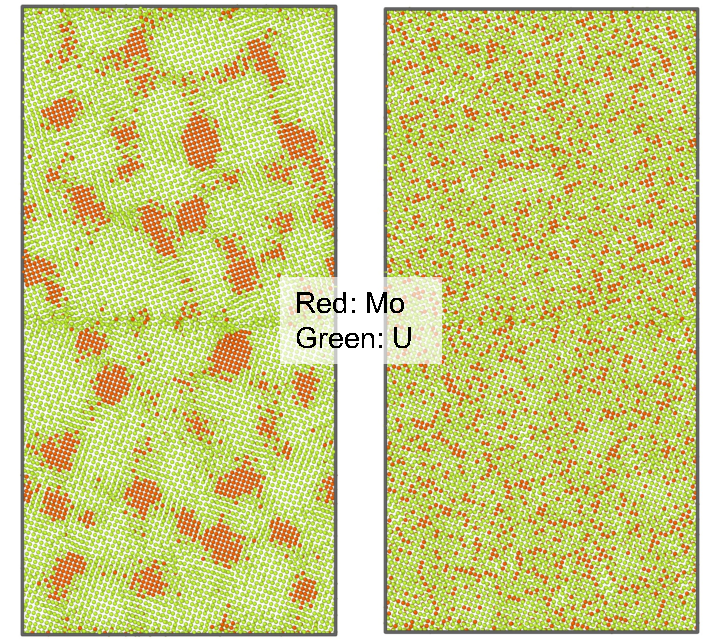
\includegraphics[width=0.6\textwidth]{Mo_precipitation.pdf} 
%DIFDELCMD <  %%%
\DIFdelendFL \DIFaddbeginFL 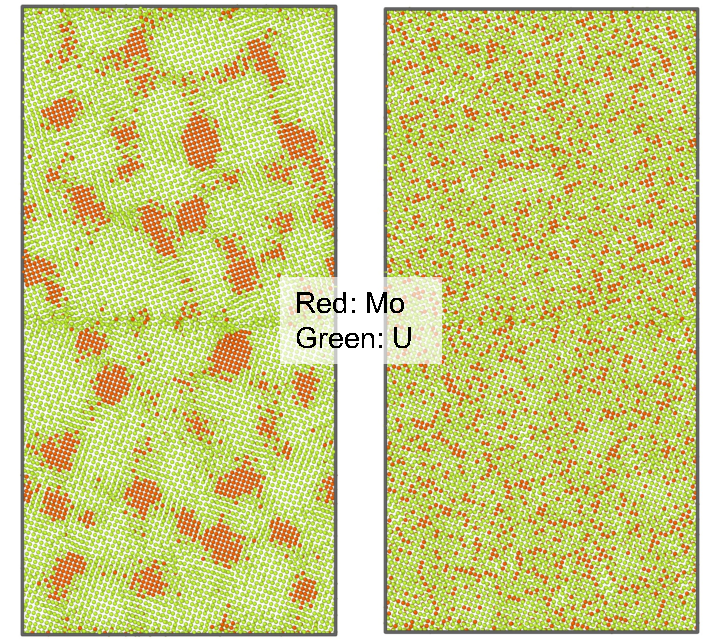
\includegraphics[width=0.6\textwidth]{Mo_precipitation} 
 \DIFaddendFL \caption{Atomic configurations from \DIFdelbeginFL \DIFdelFL{hydrid }\DIFdelendFL \DIFaddbeginFL \DIFaddFL{hybrid }\DIFaddendFL MDMC simulations at 900 K showing (\DIFdelbeginFL \DIFdelFL{a}\DIFdelendFL \DIFaddbeginFL \DIFaddFL{left}\DIFaddendFL ) Mo precipitation with the EAM potential and (\DIFdelbeginFL \DIFdelFL{B}\DIFdelendFL \DIFaddbeginFL \DIFaddFL{right}\DIFaddendFL ) stable solid solution with the ADP-type potential. }
 \label{fig:Mo_precip}
\end{figure}

The stable zone of the $\gamma$ phase is shown by the c/a ratio plotted in \DIFdelbegin \DIFdel{figure \ref{fig:c_a_ratio}}\DIFdelend \DIFaddbegin \DIFadd{\cref{fig:c_a_ratio}}\DIFaddend . The bct phase is stable when $T<650$ K and the molar fraction of Mo $c_{Mo}<0.2$. In this zone, the $c/a$ ratio increases with increasing $c_{Mo}$ and is insensitive to temperature with a weak U-shaped dependence. In contrast, the $\gamma$ phase, indicated by $c/a\approx1$, is stable when $T>650$ K or $c_{Mo}\geq0.2$. Although the bct phase is not exactly the same as the $\alpha$-U structure, and the transition temperature is lower than the actual $\alpha-\beta$ transition point of U, \DIFdelbegin \DIFdel{figure \ref{fig:c_a_ratio} }\DIFdelend \DIFaddbegin \DIFadd{\cref{fig:c_a_ratio} }\DIFaddend indicates that the potential captures the overall behavior that the $\gamma$ phase is stabilized by increasing temperature and Mo concentration. It is thereby applicable for studying the properties of U-Mo systems either with high Mo content or at high temperatures. \DIFaddbegin \DIFadd{Note that this potential was primarily developed for simulating bcc U-Mo solid solution alloys.
}\DIFaddend 

%DIF > It is known that without being able to describe the actual $\alpha-U$ and the U$_2$Mo phases, the potential is not suitable for studying the phase diagram at thermal equilibrium. 
\DIFaddbegin 

\DIFaddend \begin{figure}[h!]
 \centering
 \DIFdelbeginFL %DIFDELCMD < 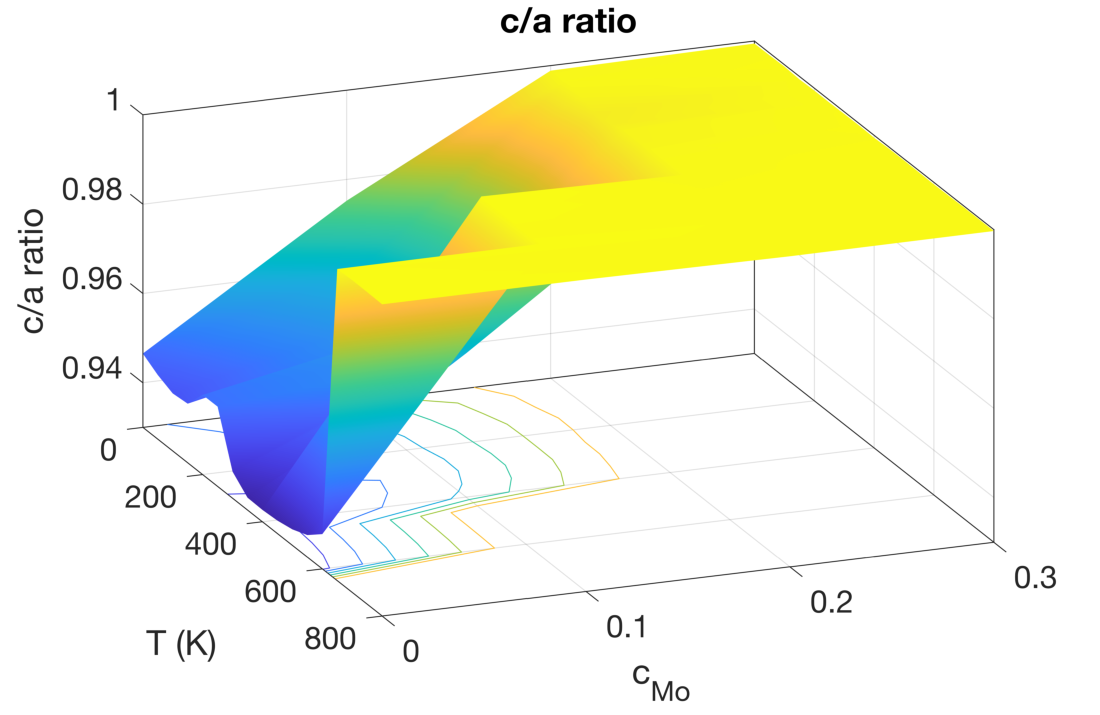
\includegraphics[width=0.8\textwidth]{c_a.pdf} 
%DIFDELCMD <  %%%
\DIFdelendFL \DIFaddbeginFL 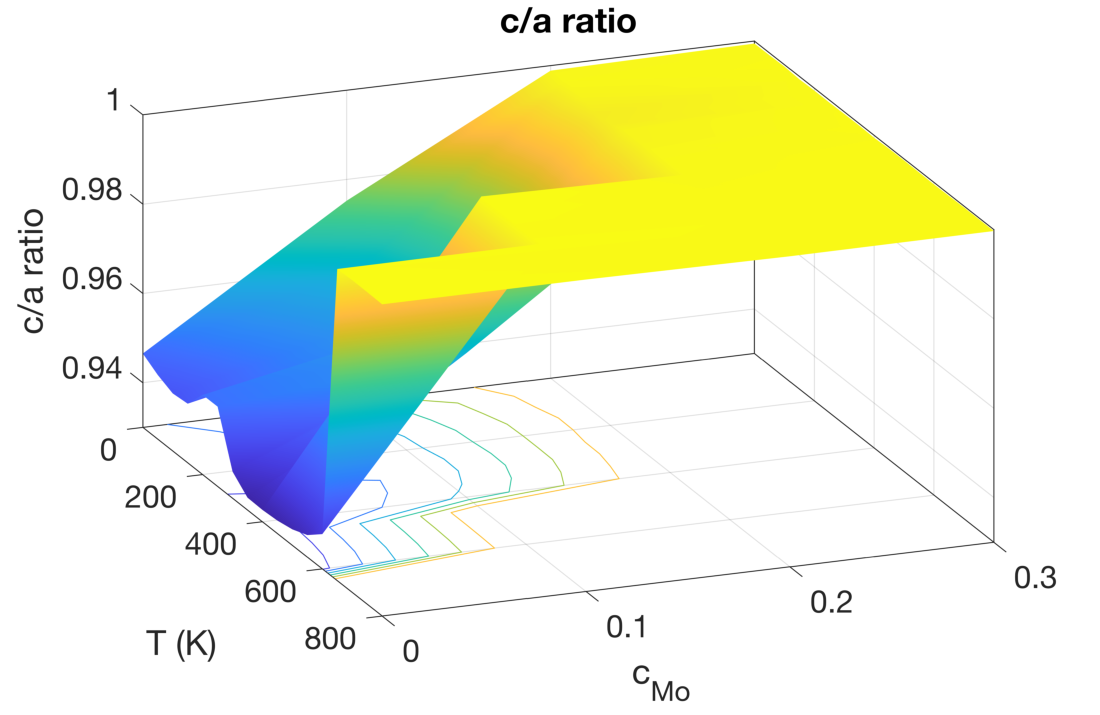
\includegraphics[width=0.8\textwidth]{c_a} 
 \DIFaddendFL \caption{The c/a ratio as a function of Mo molar fraction and temperature. \DIFaddbeginFL \DIFaddFL{The bcc solid solution phase is stable when $c_{Mo}$ is above 0.2 or $T$ is above 650 K. }\DIFaddendFL }
 \label{fig:c_a_ratio}
\end{figure}

\DIFaddbegin \DIFadd{The atomic pressure and volume were computed to investigate their dependence on the local atomic environment. The atomic pressure is computed as $\frac{1}{3}(\sigma_{xx}+\sigma_{yy}+\sigma_{zz})$, which are the normal atomic stress components computed in LAMMPS. To compute atomic volume, a Voronoi tessellation was carried out by taking the atoms as cell centers, and the cell volumes were taken as the atomic volumes. In the solid solution phase, by average, U atoms are under compression while Mo atoms are under tension, as shown in \cref{fig:vol_pressure}(a), while the overall simulation cell exhibits zero pressure at the boundaries. This is consistent with the fact that U has a larger atomic size than Mo. At room temperature, bcc U has a lattice constant of 3.47 }{\DIFadd{\AA}}\DIFadd{, versus 3.15 }{\DIFadd{\AA}} \DIFadd{for bcc Mo \cite{steiner_2016}. The atomic pressure of U atoms increases slightly in magnitude with an increasing number of 1$^{st}$ nearest neighbor (1NN) Mo atoms, showing the dependence on the local atomic environment. In U-10Mo solid solution, U atoms are found to have a larger average atomic volume than Mo, as shown in \cref{fig:vol_pressure}(b). For both, the atomic volumes decrease with an increasing number of 1NN Mo atoms almost linearly until five or six 1NN Mo atoms, for which the few data points may not warrant good statistics. The results imply that Mo-rich regions will have smaller atomic volumes than U-rich regions and are under tension. 
}

\begin{figure}[h!]
 \centering
 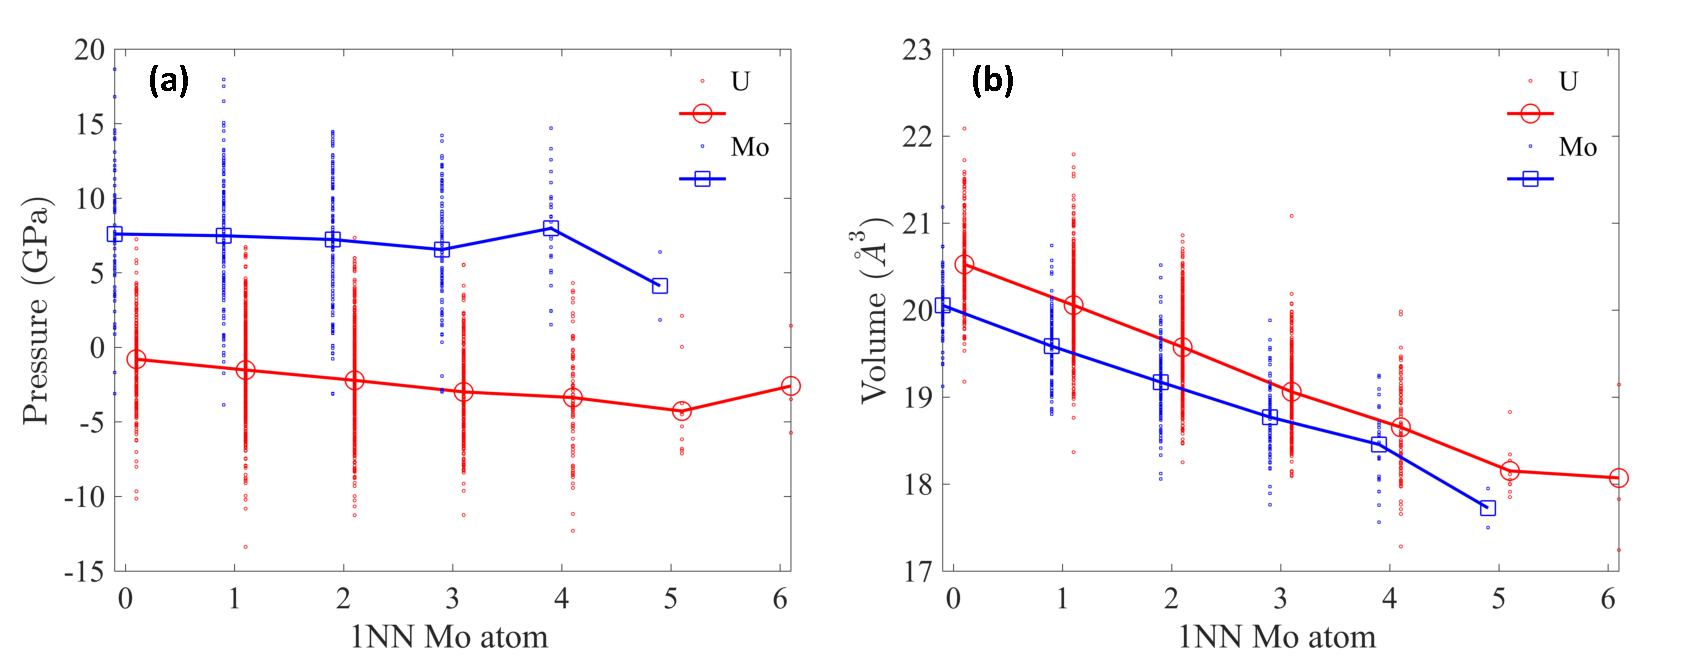
\includegraphics[width=0.8\textwidth]{vol_pressure} 
 \caption{\DIFaddFL{(a) Atomic pressure and (b) volume of U and Mo atoms as functions of 1NN Mo atoms. Positive (negative) pressure means tension (compression). Data points for Mo are shifted to the left and U to the right by 0.1 for clarity. }}
 \label{fig:vol_pressure}
\end{figure}

\begin{figure}[h!]
 \centering
 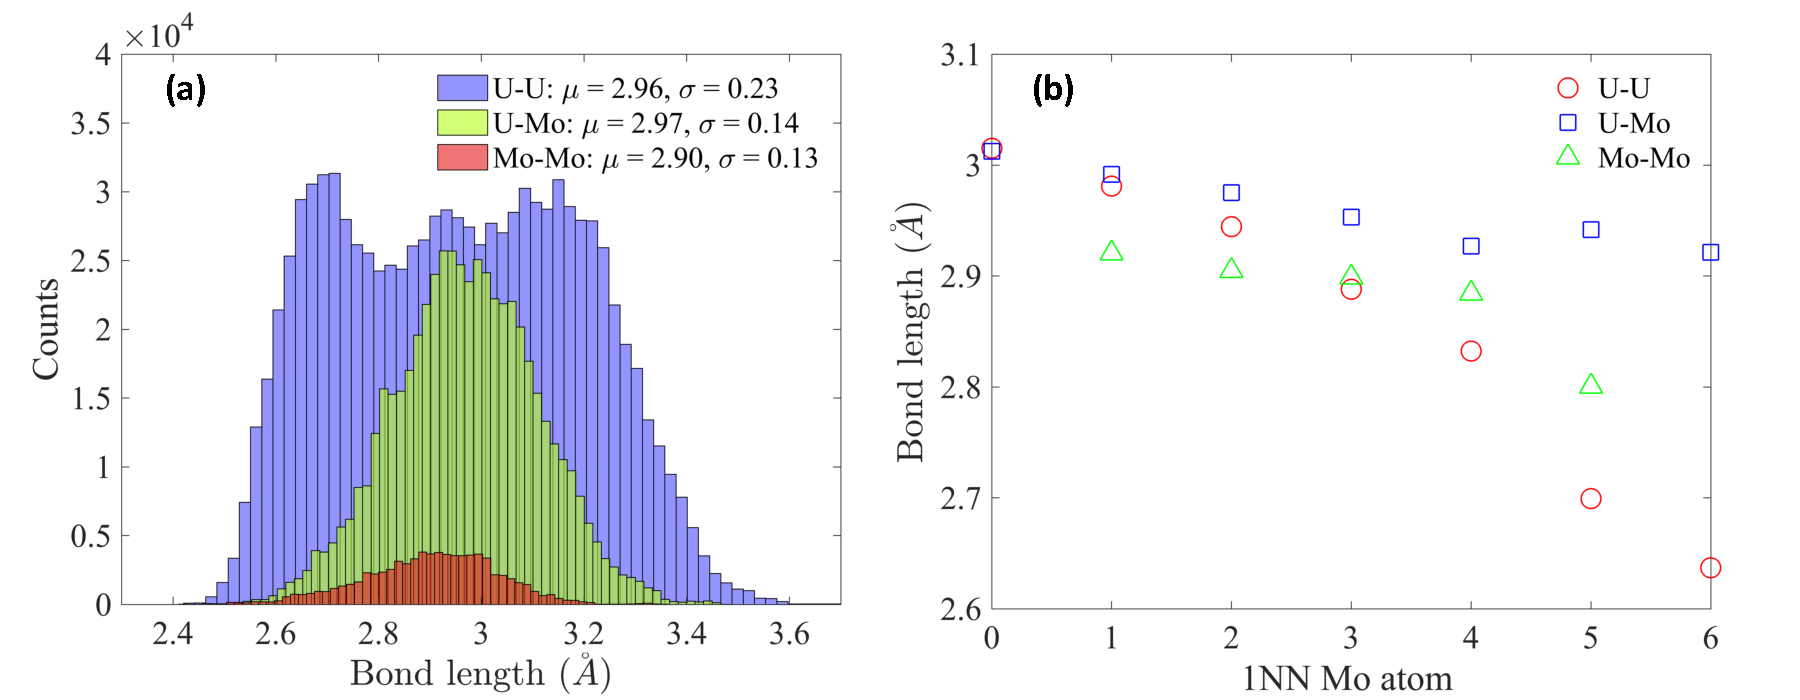
\includegraphics[width=0.8\textwidth]{bond_length} 
 \caption{\DIFaddFL{(a) Distributions of U-U, U-Mo, and Mo-Mo bond lengths, and (b) the dependence of average U-U, U-Mo, and Mo-Mo bond lengths on 1NN Mo atoms.}}
 \label{fig:bond_length}
\end{figure}

\DIFadd{The bcc lattice of U-10Mo solid solution is highly distorted, as indicated by the bond length distribution in \cref{fig:bond_length}(a). Here, 1NN bonds in a 2000 atom supercell equilibrated at 300 K were characterized. The U-U bond has the broadest distribution, with a standard deviation of $\sigma$ = 0.23 }{\DIFadd{\AA}}\DIFadd{, which is about 8\% of the mean bond length, $\mu$=2.96 }{\DIFadd{\AA}}\DIFadd{, while the range of variation spreads from 2.4 }{\DIFadd{\AA}} \DIFadd{to about 3.6 }{\DIFadd{\AA}}\DIFadd{. The U-Mo bond has the largest mean length ($\mu$=2.97 }{\DIFadd{\AA}}\DIFadd{), and the Mo-Mo bond has the smallest mean length ($\mu$=2.90 }{\DIFadd{\AA}}\DIFadd{). For the three types of bonds, the lengths decrease with an increasing number of 1NN Mo atoms, as shown in \cref{fig:bond_length}(b). In all atomic environments, U-Mo bonds have the largest average lengths. In the U-rich environment (with less than three 1NN Mo atoms), U-U bonds have larger average lengths than Mo-Mo but become shorter than Mo-Mo bonds when there are more than three 1NN Mo atoms. The U-U bonds experience the most reduction in length from U-rich to Mo-rich environments. The change in bond length is consistent with the reduction in atomic volume in \cref{fig:vol_pressure}(b). 
}

\DIFaddend \subsection{Xe substitution in U-Mo}

The vacancy formation energy $E^f_v$ and the Xe solution energy $E^s_{Xe}$ are shown in \DIFdelbegin \DIFdel{figure \ref{fig:Evf}}\DIFdelend \DIFaddbegin \DIFadd{\cref{fig:Evf}}\DIFaddend , both exhibiting \DIFdelbegin \DIFdel{a probability distribution, indicating the dependence on }\DIFdelend \DIFaddbegin \DIFadd{probability distributions, which indicates their dependence on the }\DIFaddend local atomic environment. Such a dependence is typical in concentrated alloys and implies the importance of sampling different atomic environments. The distributions were fitted using \DIFdelbegin \DIFdel{the }\DIFdelend \DIFaddbegin \DIFadd{a }\DIFaddend Gaussian distribution function based on their shapes. The mean and standard deviations obtained from the fitting are listed in \DIFdelbegin \DIFdel{Table \ref{Table:EfV} }\DIFdelend \DIFaddbegin \DIFadd{\cref{Table:EfV} }\DIFaddend along with the chemical potentials of U and Mo\DIFdelbegin \DIFdel{as well}\DIFdelend . The mean vacancy formation energy $<E^f_v>$ computed is 1.67 eV. This value is higher than the average value obtained by Jin et al. in U-20Mo (in atomic percent) at 0 K using the same ADP-type potential \cite{jin2021}, where the formation energies for U-vacancy (vacancy created by removing a U atom) and Mo-vacancy were computed to be 1.07 eV and 1.30 eV, respectively. The discrepancy may come from the different methods used for deriving the chemical potentials. In Jin et al., the \DIFdelbegin \DIFdel{potential per atom averaged }\DIFdelend \DIFaddbegin \DIFadd{average }\DIFaddend over all atoms was used for the chemical potential for both U and Mo, and in this work, the chemical potentials \DIFdelbegin \DIFdel{and }\DIFdelend \DIFaddbegin \DIFadd{of }\DIFaddend U and Mo were derived separately with a notable difference, as given in \DIFdelbegin \DIFdel{Table \ref{Table:EfV}}\DIFdelend \DIFaddbegin \DIFadd{\cref{Table:EfV}}\DIFaddend . The mean Xe solution energy is 10.29 eV, much higher than that calculated using the EAM potential, 6.1 eV \cite{Beeler2020}. 

\DIFaddbegin \DIFadd{It should be noted that vacancy formation energy and Xe solution energy as defined in \cref{Efv} and \cref{EfXe} do not depend on the types of atoms that are removed to create the vacancies, because the defected and reference cells have the same numbers of U and Mo atoms. As discussed in \cite{zhang2021,morgan2020}, the formation of a vacancy in a real material system does not involve removing an atom, although it is prescribed that way in atomistic calculations. Rather, the total mass should be conserved, as \cref{Efv} and \cref{EfXe} imply. Vacancies can be generated from sinks such as free surfaces and grain boundaries without removing any atoms, and they do not feature chemical types. In atomistic calculations, as the reference cell usually has one more atom than the defected cell, the chemical potential of the removed atom is added into the defected cell to conserve the total mass and remove the dependence of the result on the type of the removed atom. As such, there is no distinction between "U vacancies" and "Mo vacancies". There is a slight difference in composition between cells having a U atom removed and those having a Mo atom removed. Here, we assume such a negligible change in composition won’t cause a substantial change in vacancy formation energy. The insertion of Xe follows the creation of a vacancy, and the resulting Xe solution energies are independent of the type of the removed atom as well. 
}

\DIFaddend \begin{figure}[h!]
 \centering
 \DIFdelbeginFL %DIFDELCMD < 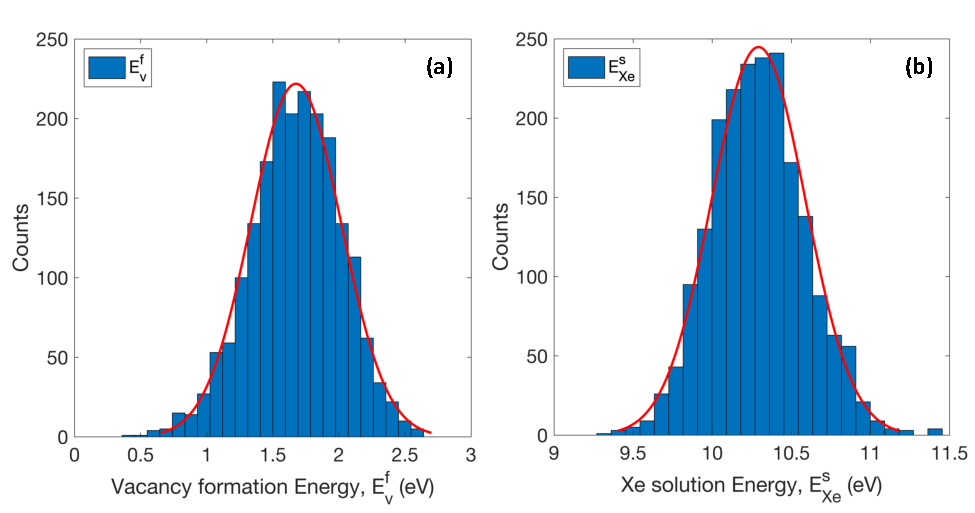
\includegraphics[width=0.8\textwidth]{EvF.pdf} 
%DIFDELCMD <  %%%
\DIFdelendFL \DIFaddbeginFL 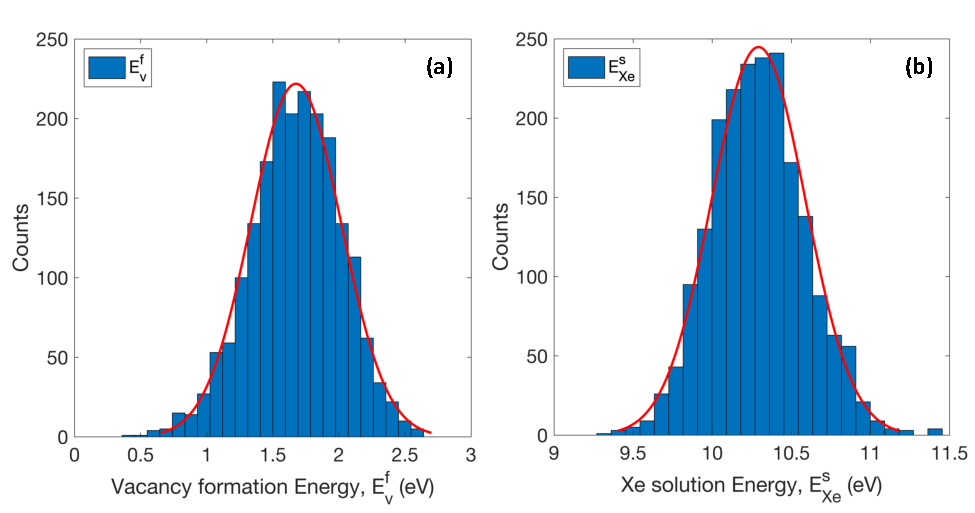
\includegraphics[width=0.8\textwidth]{EvF} 
 \DIFaddendFL \caption{Distributions of (a) vacancy formation energy and (b) Xe solution energy in U-10Mo. }
 \label{fig:Evf}
\end{figure}

\begin{table}[h!]
\centering
\begin{tabular}{|l|l|l|l|l|l|l|}
\hline
Quantity & $\mu_U$ & $\mu_{Mo}$ & $<E^f_v>$      & $<\sigma^f_v>$      & $<E^s_{Xe}>$       & $<\sigma^s_{Xe}>$      \\ \hline
Value    & -4.1125 & -6.6934     & 1.6748         & 0.3415              & 10.2924           & 0.2965 \\ \hline
\end{tabular}
\caption{Chemical potentials of U and Mo, $\mu_U$ and $\mu_{Mo}$, mean vacancy formation energy $<E^f_v>$, and the standard deviation $<\sigma^f_v>$, mean Xe solution energy, $<E^s_{Xe}>$, and the standard deviation, $<\sigma^s_{Xe}>$, in U-10Mo calculated at 300 K using molecular dynamics simulations, all in units of eV.}\label{Table:EfV}
\end{table}

The \DIFaddbegin \DIFadd{vacancy formation energy ($E^f_v$), }\DIFaddend Xe solution energy \DIFdelbegin \DIFdel{is }\DIFdelend \DIFaddbegin \DIFadd{($E^s_{Xe}$), and their difference are }\DIFaddend plotted against the numbers of \DIFdelbegin \DIFdel{1$^{st}$ nearest neighbor (}\DIFdelend \DIFaddbegin \DIFadd{Mo atoms in the }\DIFaddend 1NN \DIFdelbegin \DIFdel{) }\DIFdelend and 2NN \DIFdelbegin \DIFdel{Mo atoms in figure \ref{fig:MoNN}. It is }\DIFdelend \DIFaddbegin \DIFadd{distances in \cref{fig:MoNN}. The $E^f_v$ is found to increase very slightly with the number of 1NN Mo atoms, as shown in \cref{fig:MoNN}(a), while a clear positive correlation between $E^s_{Xe}$ and the number of 1NN Mo atoms is identified, \cref{fig:MoNN}(b). Note that $E^s_{Xe}$ as defined in \cref{EfXe} contains $E^f_{v}$. Their difference was computed and also }\DIFaddend found to increase with the number \DIFaddbegin \DIFadd{of }\DIFaddend 1NN Mo atoms, \DIFdelbegin \DIFdel{suggesting }\DIFdelend \DIFaddbegin \DIFadd{as shown in \cref{fig:MoNN}(c). The lower $E^s_{Xe}$ in a U-rich environment than in a Mo-rich environment indicates }\DIFaddend that Xe prefers \DIFaddbegin \DIFadd{to be surrounded by U atoms, and the preference is not from the environmental dependence of the $E^f_{v}$. Instead, the preference of Xe for }\DIFaddend a U-rich environment \DIFdelbegin \DIFdel{. No }\DIFdelend \DIFaddbegin \DIFadd{can be explained by the atomic volume shown in \cref{fig:vol_pressure}(b). The U-rich environment has a larger atomic volume and is therefore preferred by inert gas atoms such as Xe. In comparison, $E^f_{v}$, $E^s_{Xe}$, and their difference show no }\DIFaddend clear dependence on the number of 2NN Mo atoms\DIFdelbegin \DIFdel{can be identified, }\DIFdelend \DIFaddbegin \DIFadd{, as shown in \cref{fig:MoNN}(d)-(f), }\DIFaddend indicating that the dependence is very local within the 1NN distance. \DIFaddbegin \DIFadd{Note that for the environments with many Mo neighbors, only a few data points were collected from MD simulations in each case, and thus the averaged values are subject to large uncertainty but are included for completeness.
}\DIFaddend 

\begin{figure}[h!]
 \centering
 \DIFdelbeginFL %DIFDELCMD < 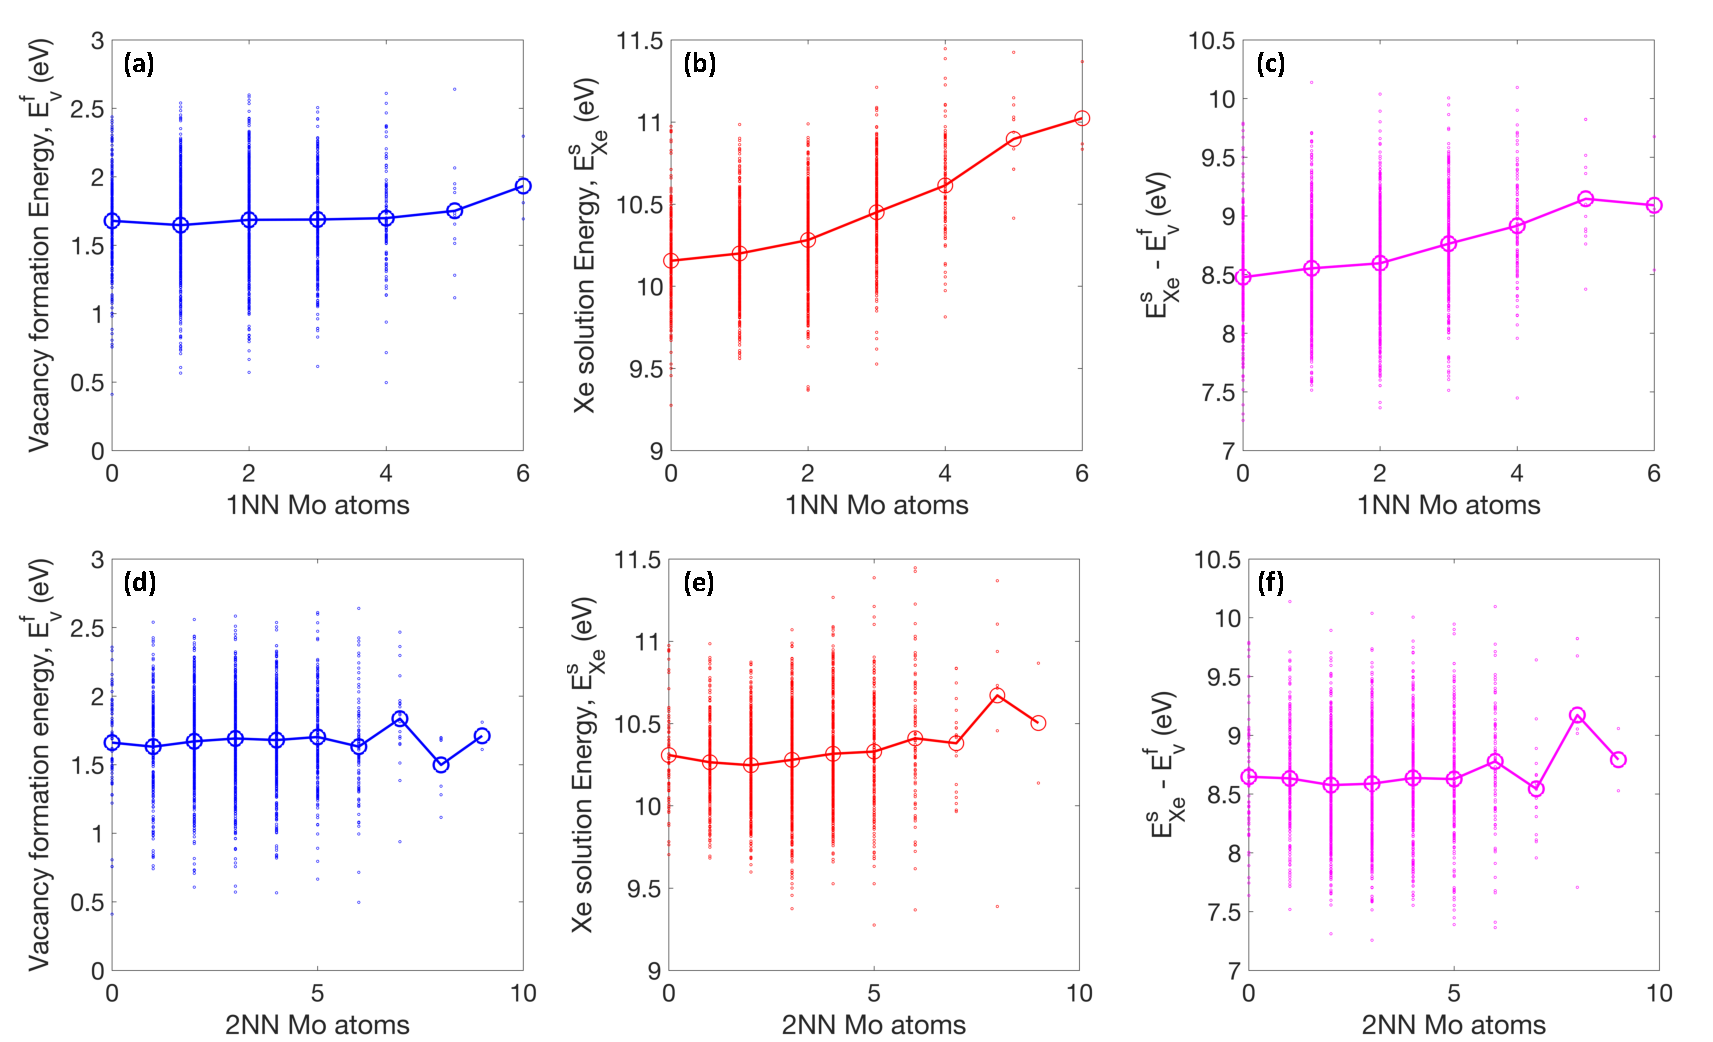
\includegraphics[width=0.8\textwidth]{MoNN.pdf} 
%DIFDELCMD <  %%%
\DIFdelendFL \DIFaddbeginFL 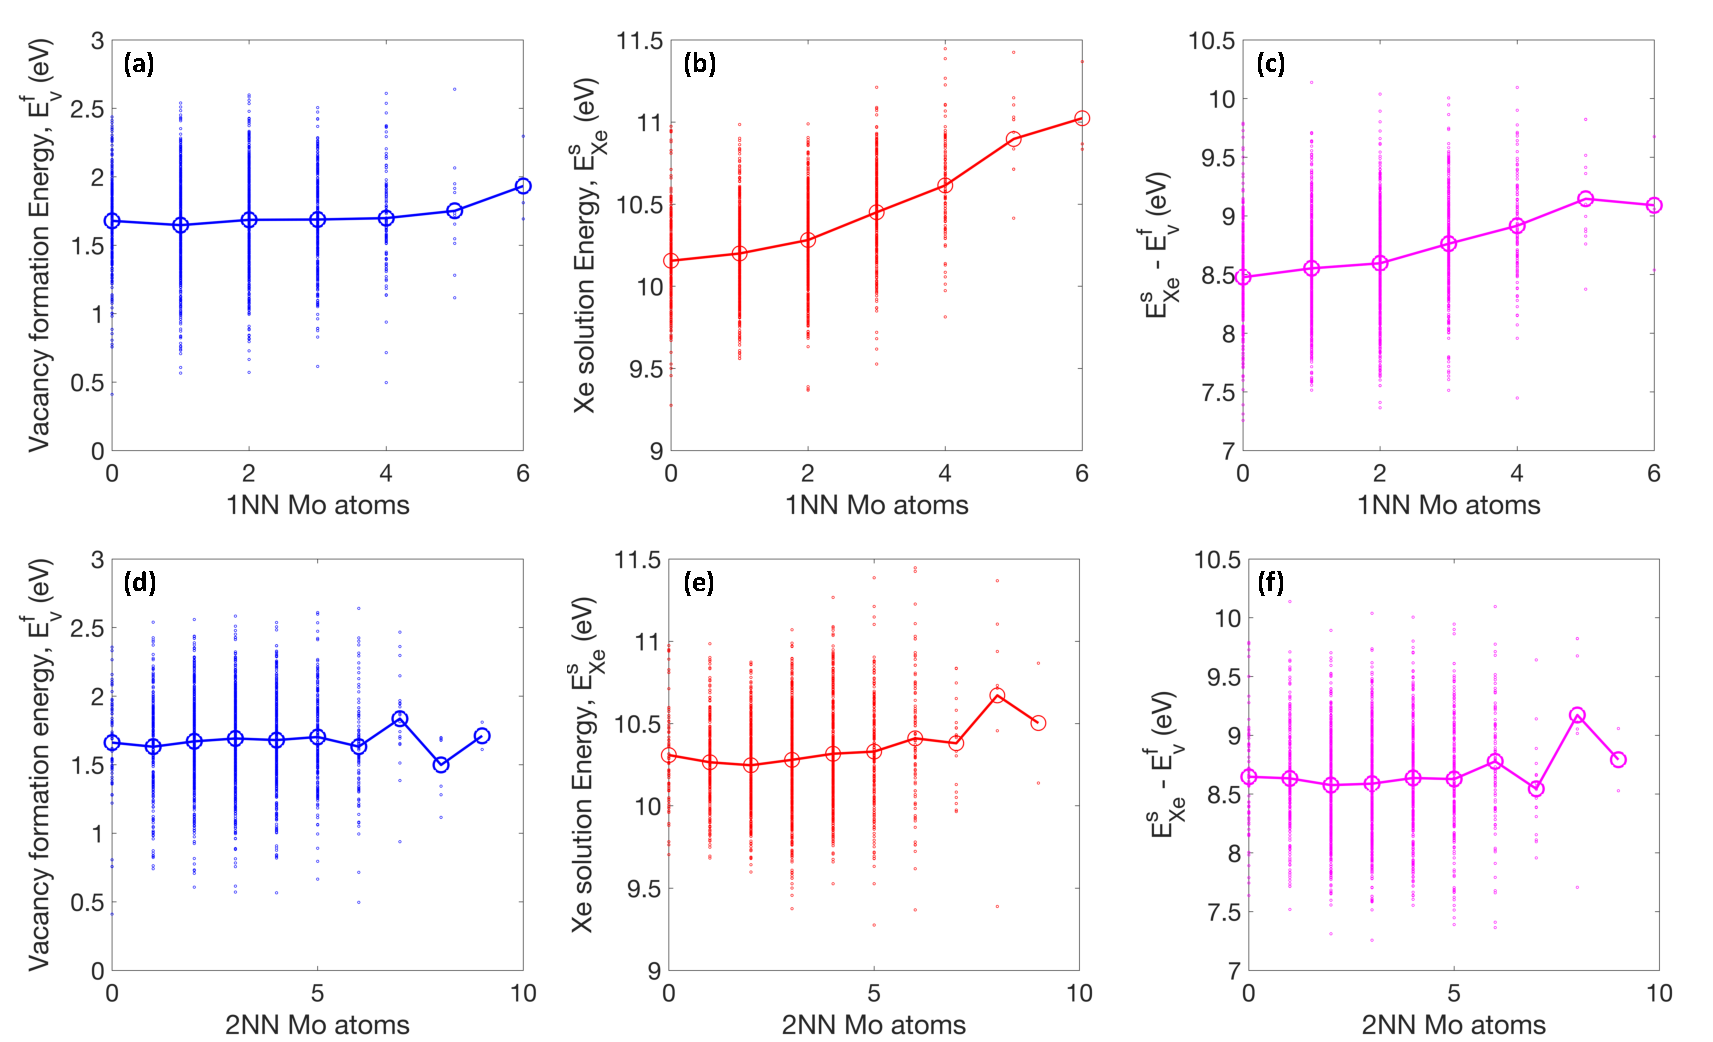
\includegraphics[width=0.8\textwidth]{MoNN} 
 \DIFaddendFL \caption{Dependence of \DIFaddbeginFL \DIFaddFL{(a) vacancy formation energy, (b) }\DIFaddendFL Xe solution energy\DIFaddbeginFL \DIFaddFL{, and (c) their difference }\DIFaddendFL on the number of \DIFdelbeginFL \DIFdelFL{(a) }\DIFdelendFL 1 \DIFdelbeginFL \DIFdelFL{$^{st}$ nearest neighbor }\DIFdelendFL \DIFaddbeginFL \DIFaddFL{NN Mo atoms. In }\DIFaddendFL (\DIFdelbeginFL \DIFdelFL{1NN}\DIFdelendFL \DIFaddbeginFL \DIFaddFL{d}\DIFaddendFL )\DIFdelbeginFL \DIFdelFL{and }\DIFdelendFL \DIFaddbeginFL \DIFaddFL{-}\DIFaddendFL (\DIFdelbeginFL \DIFdelFL{b}\DIFdelendFL \DIFaddbeginFL \DIFaddFL{f}\DIFaddendFL ) \DIFdelbeginFL \DIFdelFL{2NN }\DIFdelendFL \DIFaddbeginFL \DIFaddFL{the corresponding dependence on the number of }\DIFaddendFL Mo atoms \DIFaddbeginFL \DIFaddFL{within the 2NN distance are shown}\DIFaddendFL . \DIFaddbeginFL \DIFaddFL{The averaged values are shown by large markers connected by lines to guide the visualization. }\DIFaddendFL }
 \label{fig:MoNN}
\end{figure}

\FloatBarrier

\subsubsection{Voids and bubbles in U-Mo}

\subsection{Surface energies of voids}

In order to generate bubbles, voids of varying size must be generated. This allows for the calculation of a void surface area as a function of radius, and the surface energy can be determined from \DIFdelbegin \DIFdel{equation \ref{eq:surface}
}\DIFdelend \DIFaddbegin \DIFadd{\cref{eq:surface}
}\DIFaddend 

\begin{equation}
\label{eq:surface}
E_{surf}= \frac{(E^{*} - E)}{A} \times N
\end{equation}

\noindent where $\it{E^{*}}$ is the potential energy per atom of the system with a void, $\it{E}$ is the potential energy per atom of the perfect crystal of U-Mo, $\it{A}$ is the total surface area of the void, and $\textit{N}$ is the number of atoms in the system with a void. The void surface energy is shown in \DIFdelbegin \DIFdel{Fig. \ref{fig:voidE} }\DIFdelend \DIFaddbegin \DIFadd{\cref{fig:voidE} }\DIFaddend as a function of the void radius. 

\begin{figure}[h!]
 \centering
 \DIFdelbeginFL %DIFDELCMD < 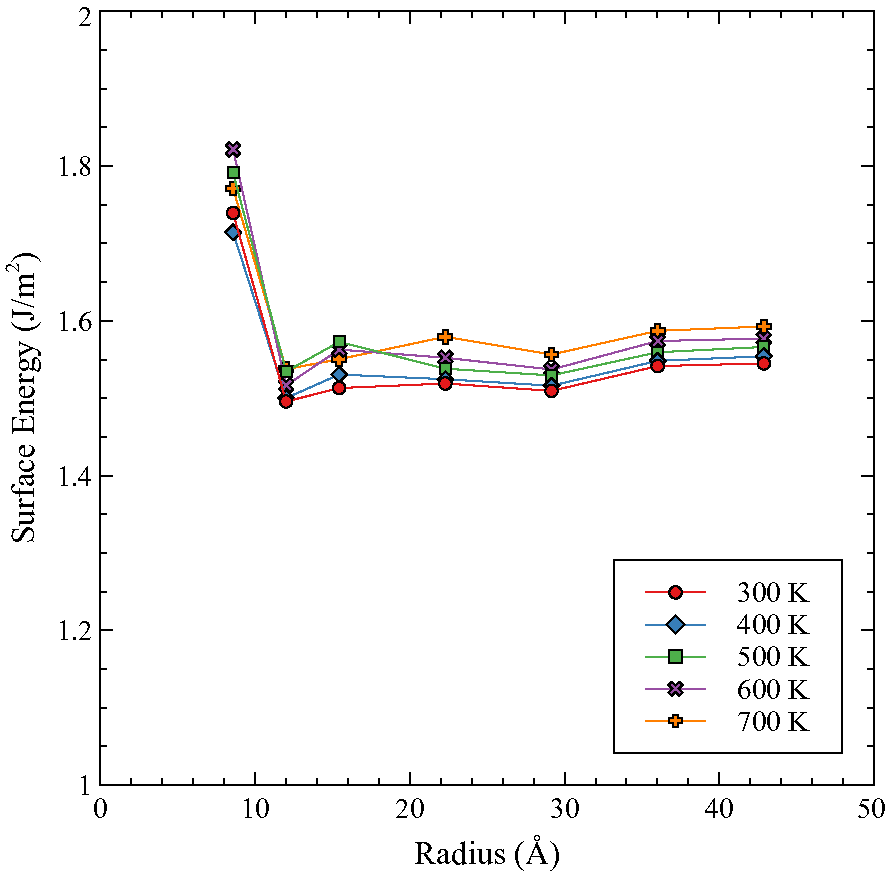
\includegraphics[width=0.7\textwidth]{Esurf.pdf} 
%DIFDELCMD <  %%%
\DIFdelendFL \DIFaddbeginFL 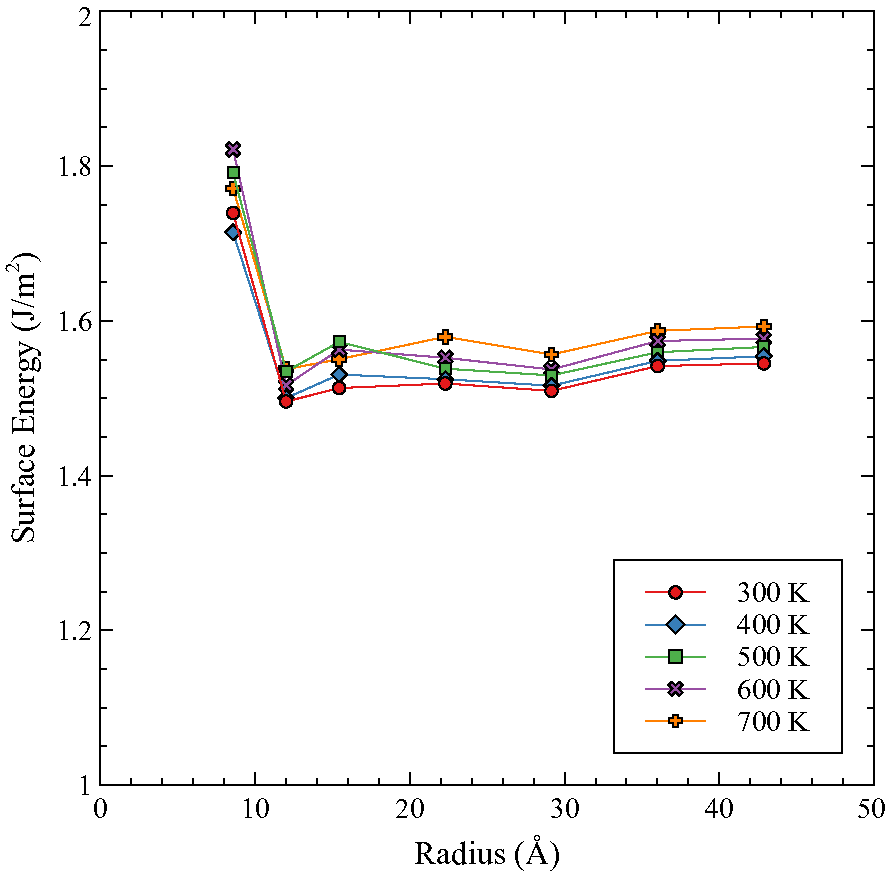
\includegraphics[width=0.7\textwidth]{Esurf} 
 \DIFaddendFL \caption{The void surface energy as a function of radius and temperature in U-10Mo.}
 \label{fig:voidE}
\end{figure}

\noindent It can be observed that the void surface energy converges above a radius of 1.5 nm for all temperatures to a value of approximately 1.5 J/m$^2$. Also, the void surface energy tends to increase slightly with increasing temperature. This is in accordance with the average surface energy for U-Mo planar surfaces as determined in \cite{beeler2018}, which utilized the Starikov ADP \cite{starikov2018}. It should be noted that the EAM potential was previously utilized to analyze void surface energy, and predicted a value 0.4 J/m$^2$ lower than the value reported here. This provides confidence in the accurate implementation of the potential \DIFdelbegin \DIFdel{, }\DIFdelend \DIFaddbegin \DIFadd{with a }\DIFaddend validation of different methodologies for obtaining average surface energies, and underlines the importance of this work to incorporate a more accurate U-Mo potential which can also describe Xe interactions. \DIFaddbegin \DIFadd{Statistical errors for the determination of surface energies are on the order of 0.04 J/m$^2$. 
}\DIFaddend 

\subsection{Xe bubble equation of state in U-Mo}

The \DIFdelbegin \DIFdel{equation of state (EOS ) }\DIFdelend \DIFaddbegin \DIFadd{EOS }\DIFaddend can be determined by tracking \DIFaddbegin \DIFadd{both }\DIFaddend the pressure inside the bubble and the bubble size as a function of the number of Xe atoms present in the bubble while the system is equilibrated in an NVT ensemble, which provides a pressure versus density relationship. This data can be fit to an EOS that provides a generalized function predicting the relationship between pressure, temperature, and molar volume. \DIFdelbegin \DIFdel{In order to extend the applicability of the EOS, temperatures }\DIFdelend \DIFaddbegin \DIFadd{Temperatures }\DIFaddend from 300 K to 700 K are analyzed \DIFdelbegin \DIFdel{, }\DIFdelend for all bubble sizes previously mentioned. 
\DIFdelbegin \DIFdel{No restrictions are imposed on the fitting parameters for each individual EOS. 
}\DIFdelend 

In line with the previous study exploring the EOS of Xe bubbles in U-Mo \cite{Beeler2020}, a Virial \DIFdelbegin \DIFdel{equation of state }\DIFdelend \DIFaddbegin \DIFadd{EOS }\DIFaddend is utilized, expanded to the third order with respect to volume and the second order with respect to temperature, as is shown in equation \DIFdelbegin \DIFdel{\ref{eq:virial}}\DIFdelend \DIFaddbegin \DIFadd{\cref{eq:virial}}\DIFaddend , 

\begin{equation}
\label{eq:virial}
P=\frac{RT}{v}\bigg( A + \frac{B}{v} + \frac{C}{v^2} + \frac{D}{v^3} \bigg)
\end{equation}

\noindent where \textit{A}=1, and \textit{B}, \textit{C}, and \textit{D} are temperature-dependent Taylor series of 1/T (\textit{B=b$_0$ + b$_1$/T + b$_2$/T$^2$}, \textit{C=c$_0$ + c$_1$/T + c$_2$/T$^2$}, and \textit{D=d$_0$ + d$_1$/T + d$_2$/T$^2$}), leading to nine unique fitting parameters. The term $R$ is the gas constant (8.3145 J/mol-K) and $v$ is the molar volume (cm$^3$/mol). The Virial equation is a general function relating pressure, molar volume, and temperature that can be directly derived from statistical mechanics \cite{virial}. \DIFaddbegin \DIFadd{No restrictions are imposed on the fitting parameters to obtain an optimized EOS. 
}\DIFaddend 

The subsequent fit, with and without molecular dynamics data, is shown in \DIFdelbegin \DIFdel{Fig. \ref{fig:MD_Vir} and Fig. \ref{fig:Vir}}\DIFdelend \DIFaddbegin \DIFadd{\cref{fig:MD_Vir} and \cref{fig:Vir}}\DIFaddend , respectively. \DIFaddbegin \DIFadd{As expected, with higher temperatures, the pressure at a given molar volume is higher, resulting in an effective rightward shift of the data as the temperature is increased. All data with molar volumes below 500 cm$^3$/mol are displayed in \cref{fig:MD_Vir}. }\DIFaddend The MD data is removed in \DIFdelbegin \DIFdel{Fig. \ref{fig:Vir} }\DIFdelend \DIFaddbegin \DIFadd{\cref{fig:Vir} }\DIFaddend and the optimized EOS is displayed on a log/linear scale to emphasize the differences between the individual isotherms. \DIFaddbegin \DIFadd{As stated, temperature shifts the pressure to a larger value at a given molar volume, and the optimized Virial EOS accurately captures this behavior. }\DIFaddend The optimized coefficients are shown in \DIFdelbegin \DIFdel{Table \ref{tab:virial}}\DIFdelend \DIFaddbegin \DIFadd{\cref{tab:virial}}\DIFaddend . 

\begin{figure}[h!]
 \centering
 \DIFdelbeginFL %DIFDELCMD < 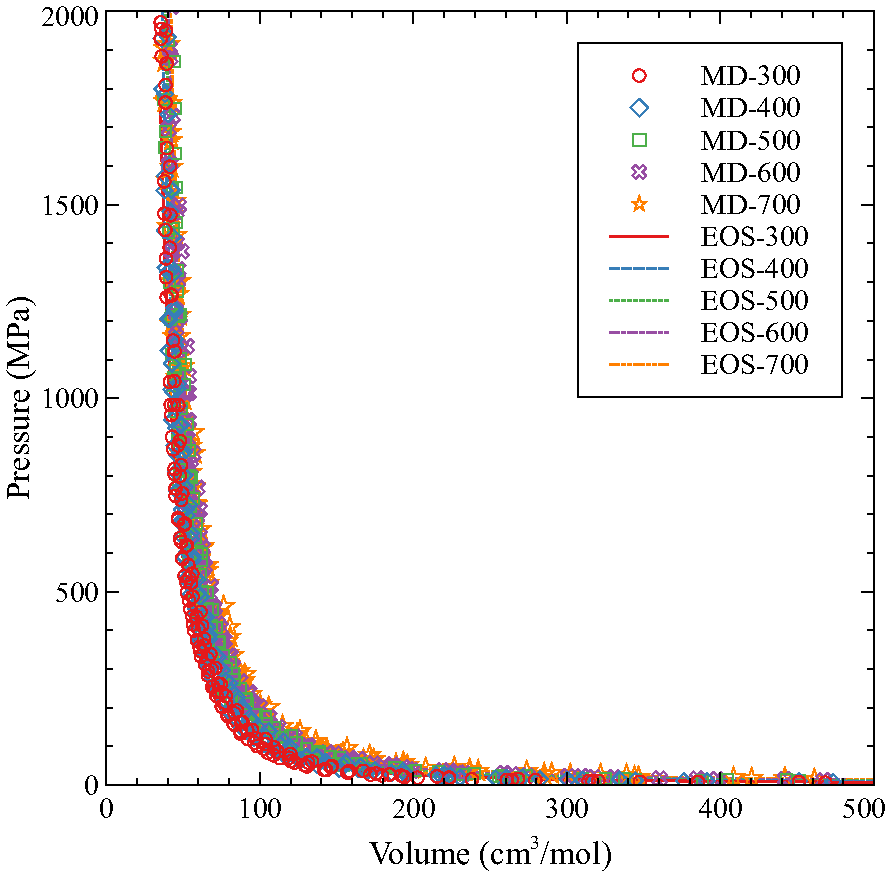
\includegraphics[width=0.8\textwidth]{MD_Virial.pdf} 
%DIFDELCMD <  %%%
\DIFdelendFL \DIFaddbeginFL 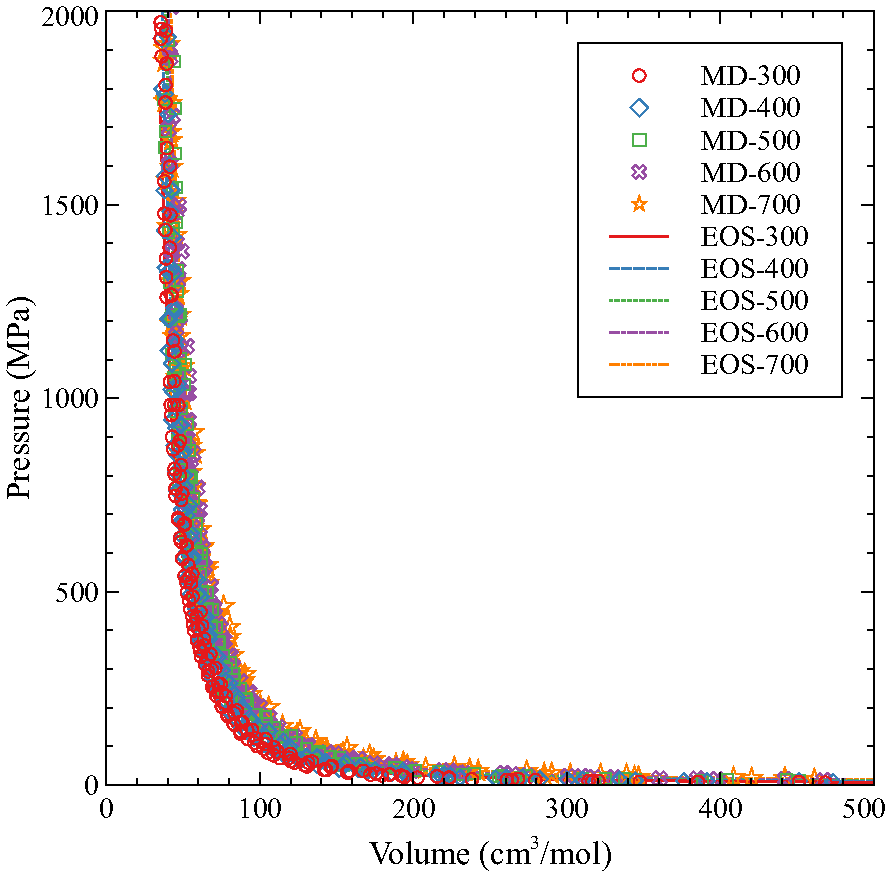
\includegraphics[width=0.8\textwidth]{MD_Virial} 
 \DIFaddendFL \caption{An \DIFdelbeginFL \DIFdelFL{equation of state (}\DIFdelendFL EOS \DIFdelbeginFL \DIFdelFL{) }\DIFdelendFL based on a virial expansion for Xe bubbles in U-10Mo from \DIFdelbeginFL \DIFdelFL{400 }\DIFdelendFL \DIFaddbeginFL \DIFaddFL{300 }\DIFaddendFL K to 700 K \DIFdelbeginFL \DIFdelFL{(a) }\DIFdelendFL compared to molecular dynamics data\DIFdelbeginFL \DIFdelFL{and (b) without molecular dynamics data}\DIFdelendFL . }
 \label{fig:MD_Vir}
\end{figure}

\begin{figure}[h!]
 \centering
 \DIFdelbeginFL %DIFDELCMD < 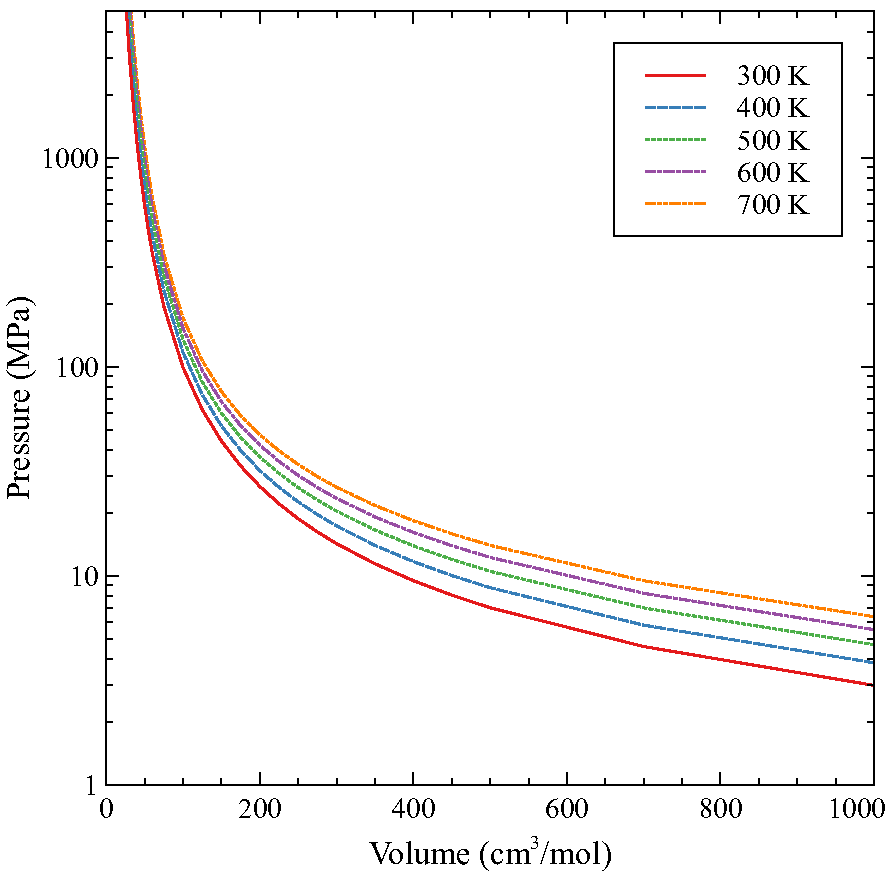
\includegraphics[width=0.8\textwidth]{virial_fit.pdf} 
%DIFDELCMD <  %%%
\DIFdelendFL \DIFaddbeginFL 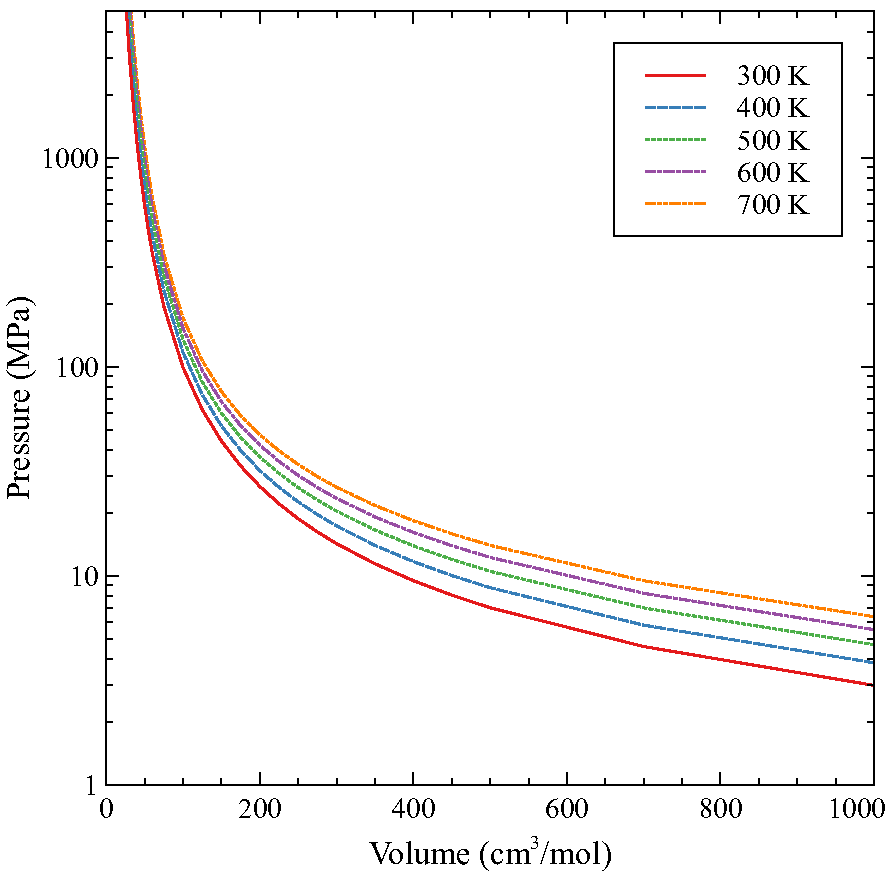
\includegraphics[width=0.8\textwidth]{virial_fit} 
 \DIFaddendFL \caption{An \DIFdelbeginFL \DIFdelFL{equation of state (}\DIFdelendFL EOS \DIFdelbeginFL \DIFdelFL{) }\DIFdelendFL based on a Virial expansion for Xe bubbles in U-10Mo from \DIFdelbeginFL \DIFdelFL{400 }\DIFdelendFL \DIFaddbeginFL \DIFaddFL{300 }\DIFaddendFL K to 700 K \DIFdelbeginFL \DIFdelFL{(a) compared to molecular dynamics data and (b) }\DIFdelendFL without molecular dynamics data. }
 \label{fig:Vir}
\end{figure}

\begin{table}[h!]
\caption{Virial \DIFdelbeginFL \DIFdelFL{equation of state }\DIFdelendFL \DIFaddbeginFL \DIFaddFL{EOS }\DIFaddendFL (\DIFdelbeginFL \DIFdelFL{Eq. \ref{eq:virial}}\DIFdelendFL \DIFaddbeginFL \DIFaddFL{\cref{eq:virial}}\DIFaddendFL ) parameters for Xe bubbles in U-Mo.}
\label{tab:virial}
\begin{center}
\begin{tabular}{|c|c|}
     \hline
      Parameter & Value \\
     \hline
     \textit{b$_0$} & 14.625 cm$^3$/mol \\
     \textit{b$_1$} & 54597.728 cm$^3$-K/mol  \\
     \textit{b$_2$} & -386.344 cm$^3$-K$^2$/mol \\
     \textit{c$_0$} & 2968.616 cm$^6$/mol$^2$ \\
     \textit{c$_1$} & 2938.010 cm$^6$-K/mol$^2$  \\
     \textit{c$_2$} & -84.545 cm$^6$-K$^2$/mol$^2$ \\
     \textit{d$_0$} & 705527.001 cm$^9$/mol$^3$ \\
     \textit{d$_1$} & 53.609 cm$^9$-K/mol$^3$ \\
     \textit{d$_2$} & 421.138 cm$^9$-K$^2$/mol$^3$ \\
     \hline
\end{tabular}
\end{center}
\label{default}
\end{table}%

While 4th order optimizations both including and excluding the 3rd order term were pursued, as has recently been performed by Yang \cite{yang2022} for Xe in UO$_2$, the accuracy of the fit to the MD data was not improved. A comparison to the Kaplun EOS \cite{Kaplun2003} is shown in \DIFdelbegin \DIFdel{Fig. \ref{fig:kap_comp}. Kaplun fit }\DIFdelend \DIFaddbegin \DIFadd{\cref{fig:kap_comp} for 400 K and 700 K. Kaplun developed }\DIFaddend a unified EOS for liquid, gas, and fluid defined from thermodynamic equations which shows excellent agreement with experimental data for a number of species. \DIFdelbegin \DIFdel{Fig. \ref{fig:kap_comp} }\DIFdelend \DIFaddbegin \DIFadd{The comparison in \cref{fig:kap_comp} }\DIFaddend shows that at low densities, the Kaplun data and the fit to the computational data converge, with the computational EOS predicting a very slightly higher pressure \DIFdelbegin \DIFdel{. At }\DIFdelend \DIFaddbegin \DIFadd{($<$0.2 MPa). The differences observed in \cref{fig:kap_comp} are exaggerated due to the log/linear scale utilized in the graphical representation. However, at }\DIFaddend high densities and high pressures, there is a dramatic difference between the Kaplun EOS and the Virial EOS from this work, indicating the importance of taking into account the U-Mo matrix for the properties of Xe bubbles. Thus, this updated Virial EOS in \DIFdelbegin \DIFdel{equation \ref{eq:virial} and Table \ref{tab:virial} }\DIFdelend \DIFaddbegin \DIFadd{\cref{eq:virial} and \cref{tab:virial} }\DIFaddend can be utilized to describe both high and low density/pressure bubbles in U-Mo over the prescribed temperature ranges. \DIFaddbegin \DIFadd{Unfortunately, there is no experimental data to base a comparison or to establish the ultimate accuracy of the EOS of Xe bubbles in U-Mo at high pressures and densities. Thus, we argue that the convergence to a pure Xe gas at low densities, and the specific incorporation of the accurate interaction between U, Mo, and Xe at high densities, provides a reasonable prediction for Xe bubble behavior in the U-Mo system. 
}\DIFaddend 

\begin{figure}[h!]
 \centering
 \DIFdelbeginFL %DIFDELCMD < 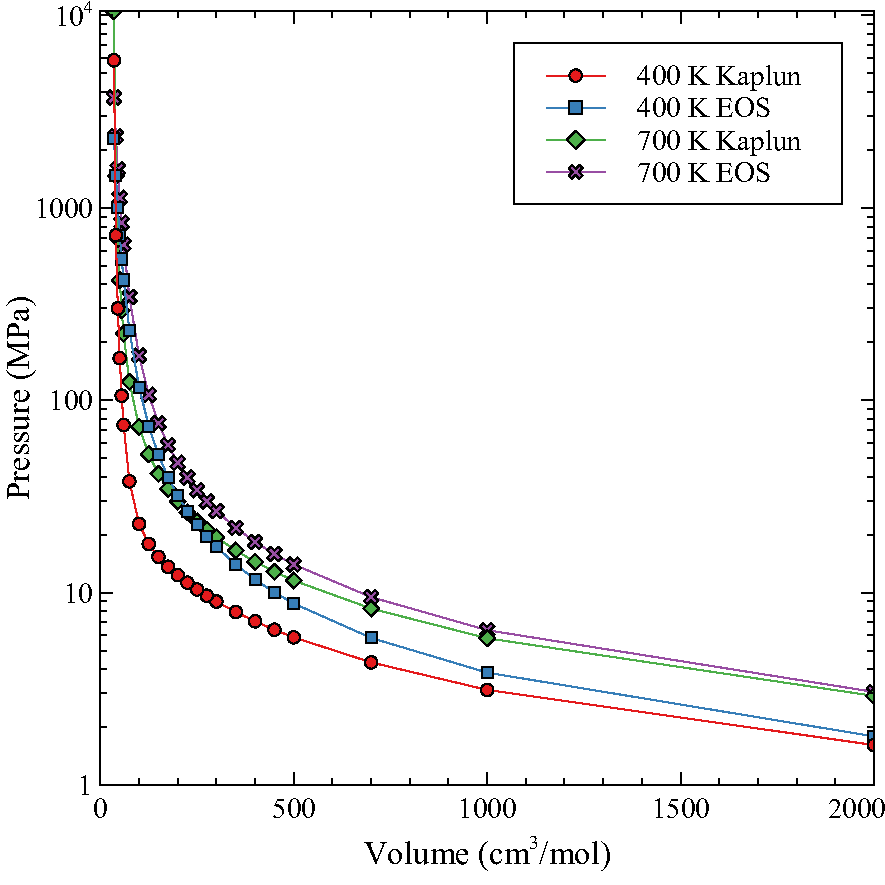
\includegraphics[width=0.7\textwidth]{kaplun_comp.pdf} 
%DIFDELCMD <  %%%
\DIFdelendFL \DIFaddbeginFL 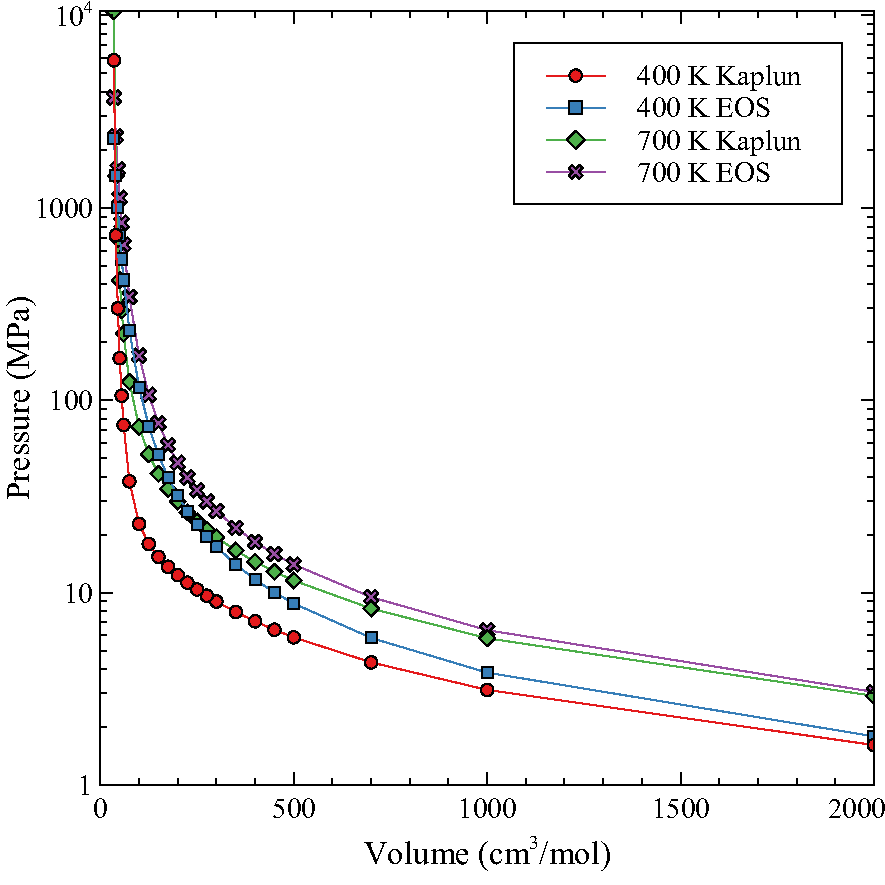
\includegraphics[width=0.7\textwidth]{kaplun_comp} 
 \DIFaddendFL \caption{Comparison between the Kaplun unified EOS (Kaplun) and the Virial EOS from this work (EOS) over a wide range of molar volumes at 400 K and 700 K.}
 \label{fig:kap_comp}
\end{figure}


\FloatBarrier

\section{Conclusions}

In this work, prior interatomic potentials for the U-Mo and the U-Mo-Xe system were reconciled under a single ADP framework, generating a novel ternary potential that utilizes the most accurate descriptions of the individual pair systems which exist. The phase stability of the $\gamma$ phase of U-Mo was explored via MDMC simulations, demonstrating the inability of prior potential forms to correctly predict the stable solid solution behavior of the alloy. The distortion of the $\gamma$ phase into a bct structure was analyzed as a function of temperature and composition, agreeing with experimental observations of bcc instability of U-rich systems at lower temperatures. A rigorous approach to vacancy and Xe substitutional energies was applied to this system for the first time, identifying key inaccuracies in previous potential formalisms and providing information on the effect of the local environment on the behavior of Xe substitutionals. Finally, voids and bubbles were explored in U-10Mo, verifying previous studies of void surface energy and providing a new equation of state for Xe bubbles specific to the U-Mo system. \DIFdelbegin \DIFdel{This work has served to demonstrate the need for an updated interatomic potential, and provided that tool, which }\DIFdelend \DIFaddbegin \DIFadd{While further experimental validations are needed to justify the accuracy of the reconciled potential, this work enables studying Xe gas behavior and gas bubble properties in U-Mo solid solutions using molecular dynamics simulations. It allows for the exploration of critical phenomena related to Xe gas atoms and bubbles in U-Mo fuel and }\DIFaddend will serve to inform mesoscale and engineering scale fuel performance simulations \DIFdelbegin \DIFdel{, providing increased accuracy and reducing known errors, allowing for the exploration of critical phenomena in U-Mo fuels}\DIFdelend \DIFaddbegin \DIFadd{with better reliability than existing interatomic potentials}\DIFaddend .

\section{Acknowledgement}
This work was supported by the U.S. Department of Energy, Office of Material Management and Minimization, National Nuclear Security Administration, under DOE-NE Idaho Operations Office Contract DE-AC07-05ID14517. This manuscript has been authored by Battelle Energy Alliance, LLC with the U.S. Department of Energy. The publisher, by accepting the article for publication, acknowledges that the U.S. Government retains a nonexclusive, paid-up, irrevocable, worldwide license to publish or reproduce the published form of this manuscript, or allow others to do so, for U.S. Government purposes. This research made use of the resources of the High-Performance Computing Center at Idaho National Laboratory, which is supported by the Office of Nuclear Energy of the U.S. Department of Energy and the Nuclear Science User Facilities.

%\section{References}

\bibliography{beelerbib}


\end{document} 
